% !Mode:: "TeX:UTF-8"
%\documentclass[twocolumn]{sig-alternate}
\documentclass[letterpaper, twocolumn,fleqn]{sig-alternate-10pt}
%\documentclass[twocolumn,10pt]{infocom}
%\documentclass[twocolumn,10pt]{IEEEtran_v15}
%\documentclass[twocolumn,10pt]{IEEEtran}
%\documentclass[twocolumn,10pt]{article}
%\usepackage[sort,nocompress,space]{cite}
%\documentclass{sig-alternate-10pt}
%\documentclass[letterpaper,twocolumn,10pt]{article}
\usepackage{epsfig,endnotes}
%\usepackage[letterpaper]{geometry}

\usepackage[export]{adjustbox}
\usepackage{tabularx}

%\usepackage{ifpdf}
%\ifpdf
%\setlength{\pdfpagewidth}{8.5in}
%\setlength{\pdfpageheight}{11in}
%\else
%\fi

%%%%%%%%%%%%%%%%%%%%%%
% Set Compact Mode   %
%%%%%%%%%%%%%%%%%%%%%%

%\newcommand{\subparagraph}{}


%\usepackage[compact]{titlesec}
%\titlespacing{\section}{0pt}{*0}{*0}
%\titlespacing{\subsection}{0pt}{*0}{*0}
%\titlespacing{\subsubsection}{0pt}{*0}{*0}
%\setlength{\parskip}{0pt}
%\setlength{\parsep}{0pt}
%\setlength{\headsep}{0pt}
%\setlength{\topskip}{0pt}
%\setlength{\topmargin}{0pt}
%\setlength{\topsep}{0pt}
%\setlength{\partopsep}{0pt}
%\setlength{\itemsep}{0pt}

%%%%%%%%%%%%%%%%%%%%%%
%
%%%%%%%%%%%%%%%%%%%%%%


\usepackage{url}
\usepackage[sort,space]{cite}
\usepackage{lineno}
\renewcommand\linenumberfont{\normalfont\bfseries\small}
\usepackage{pifont}
\usepackage{epsfig,epsf,url,amssymb}
\usepackage{tabularx}
%\usepackage{algorithm2e}
\usepackage[ruled,vlined]{algorithm2e}
\usepackage{algpseudocode}
\usepackage{amsmath}
\usepackage{mathtools}
\newtheorem{mydef}{Definition}
\usepackage{rotating}
\usepackage{wrapfig}
\usepackage{times}
\long\def\comment#1{}
\usepackage{multirow}
\usepackage{lscape}
\usepackage{stmaryrd}
\usepackage{wrapfig}
\usepackage{hhline}
\usepackage{textcomp,booktabs}
\usepackage[usenames,dvipsnames]{color}
\usepackage{colortbl}
\usepackage{multirow}
\usepackage{rotating}
\usepackage{epstopdf}
%\usepackage{hyperref}
\usepackage{url}
\definecolor{mygray}{gray}{.9}
\definecolor{mypink}{gray}{.9}
\definecolor{mycyan}{cmyk}{.3,0,0,0}

\usepackage{graphicx}
%\usepackage{subfigure}
\usepackage{subfig}
\usepackage[font=bf]{caption}

%\newcommand{\bbR}{\mathbb{R}}
%\newcommand{\calN}{\mathcal{N}}
%\newcommand{\calR}{\mathcal{R}}
%\newcommand{\calV}{\mathcal{V}}
%\newcommand{\eg}{{\it e.g.}}
%\newcommand{\etal}{{\it et al.~}}
%\newcommand{\etc}{{\it etc.}}
%\newcommand{\ie}{{\it i.e.}}
%\newcommand{\tablecapspace}{{\vspace{-0.1in}}}
%\newcommand{\tablespace}{{\vspace{-0.05in}}}
%\newcommand{\picspace}{{\vspace{-0.1in}}}
%\renewcommand{\baselinestretch}{1}
%\renewcommand{\arraystretch}{1.05}      % make the space between tabular lines larger
%\newcommand{\capspace}{}           % control space between figure/table and caption

\def\TODO#1{\textcolor{red}{}}
%\setlength{\textheight}{9.3in}
%\setlength{\columnsep}{1.4pc}
%\setlength{\textwidth}{7.1in}

\newcommand{\sys}{{\textrm{XPath}}\xspace}

\newcommand{\paragraphb}[1]{\vspace{0.05in}\noindent{\bf #1}}

\newcommand{\paraspace}{\vspace{0.05in}}
\newcommand{\parab}[1]{\paraspace\noindent{\bf #1} }
\newcommand{\parae}[1]{\paraspace\noindent{\em #1} }
\newcommand{\parabe}[1]{\paraspace\noindent{\bf \em #1} }
%\newcommand{\kai}[1]{{\color{blue}[Kai: #1]}}
\newcommand{\todo}{\textcolor{red}}

\def\naive{na\"\i ve}

\newcommand{\tabincell}[2]{\begin{tabular}{@{}#1@{}}#2\end{tabular}}

\newcommand{\subcaption}[1]{\centerline{#1}\vspace{0.1in}}
\long\def\comment#1{}
\newtheorem{theorem}{Theorem}
\newtheorem{lemma}[theorem]{Lemma}
\newtheorem{proposition}[theorem]{Proposition}
\newtheorem{corollary}[theorem]{Corollary}
%\newtheorem{problem}[theorem]{Problem}

\newenvironment{definition}[1][Definition]{\begin{trivlist}
\item[\hskip \labelsep {\bfseries #1}]}{\end{trivlist}}
\newenvironment{problem}[1][]{\begin{trivlist}
\item[\hskip \labelsep {\bfseries}]}{\end{trivlist}}
\newenvironment{remark}[1][Remark]{\begin{trivlist}
\item[\hskip \labelsep {\bfseries #1}]}{\end{trivlist}}

\newenvironment{icompact}{
  \begin{list}{$\bullet$}{
    \parsep 1pt plus 1pt
    \partopsep 1pt plus 1pt
    \topsep 1pt plus 2pt minus 1pt
    \itemsep 1.5pt plus 1pt
    \parskip 0pt plus 2pt
    \leftmargin 0.15in}
       }
  {\normalsize\end{list}}

\newenvironment{ecompact}{
  \begin{list}{$\bullet$}{
    \parsep 1pt plus 1pt
    \partopsep 1pt plus 1pt
    \topsep 1pt plus 2pt minus 1pt
    \itemsep 1.5pt plus 1pt
    \parskip 0pt plus 2pt
    \leftmargin 0.15in}
       }
  {\normalsize\end{list}}

%\hyphenpenalty=5000 %\tolerance=1000

%\hyphenation{Mega-Switch para-digm}


%%%%%%%% to calculate the time %%%%%%%%%%%%%%%%%%%%%%%%%%%%
\newcount\hour \newcount\minute
\hour=\time  \divide \hour by 60
\minute=\time
\loop \ifnum \minute > 59 \advance \minute by -60 \repeat
\def\drafttime{\ifnum \hour<13 \number\hour:%
                      \ifnum \minute<10 0\fi
                      \number\minute
                      \ifnum \hour<12 \ AM\else \ PM\fi
         \else \advance \hour by -12 \number\hour:%
                      \ifnum \minute<10 0\fi
                      \number\minute \ PM\fi}
\def\timestamp{\today \ \drafttime}

\begin{document}
%\conferenceinfo{SIGCOMM,} {XXXXXX, XXXXX, XXXXX, XXXXX.} %
%\CopyrightYear{2009} \crdata{1-59593-308-5/06/0009}

\title{TTL-based Buffer Management Scheme for Deadlock Prevention}
\maketitle

%\vspace{-0.2in}
%\begin{abstract} Remote Direct Memory Access over Converged Ethernet (RoCE) deployments
		are vulnerable to deadlocks induced by Priority Flow Control (PFC).
		Prior solutions for deadlock prevention either require significant
		changes to routing protocols, or require excessive buffers in the
		switches. In this paper, we propose a scheme for deadlock prevention,
		called \sysname{}. It does not require any changes to the routing
		protocol, and needs only modest buffers.  \sysname{} is based on the
		insight that given a set of expected lossless routes, a simple tagging
		scheme can be developed to ensure that no deadlock will occur under any
		failure conditions. We design such a scheme, prove that it prevents
		deadlock and implement it efficiently on commodity hardware.
\end{abstract}

%\vspace{-0.1in}
\section{Introduction}
\label{sec:intro}

Public cloud providers like Microsoft and Google are deploying Remote Direct
Memory Access (RDMA) over Ethernet (RoCE) in their data centers to enable low
latency, high throughput data transfers with minimal CPU
overhead~\cite{dcqcn,timely}. Systems like Pilaf~\cite{pilaf}, Farm~\cite{farm},
TesnorFlow~\cite{tensorflow}, and CNTK~\cite{cntk} rely on RDMA/RoCE for
enhanced performance. 

RoCE uses Priority Flow Control (PFC) to prevent packet drops due to buffer
overflow at the switches. PFC allows a switch to temporarily pause its upstream
neighbor. While PFC is effective, it can lead to
deadlocks~\cite{rdmaatscale,tcpbolt,hu2016deadlocks}. Deadlocks are caused by
circular buffer dependency (CBD)~\cite{hu2016deadlocks}, {\em i.e.,} the occupied 
buffers are waiting for each other in a loop.

While CBD can be caused by a routing loop, routing loop is not required -- flows
that travel on loop-free paths can create buffer dependencies that lead to CBD.
A simple but contrived example is shown in Figure~\ref{fig:basic_deadlock}. We
will discuss more realistic scenarios (e.g. Figure~\ref{fig:clos_1_bounce})
later.  See~\cite{hu2016deadlocks} for several other examples. 

The deadlock problem is not merely theoretical -- our conversations with
engineers at large cloud providers confirm that they have seen the problem in
practice and at least one provider has reported it publicly~\cite{rdmaatscale}.
Deadlock is a serious problem because a deadlock is not transient -- once a
deadlock forms, it does not go away even after the conditions (e.g. a temporary
routing loop due to link failure) that caused its formation have
abated~\cite{rdmaatscale}. Worse, a small initial deadlock may cause the PFC
frames to propagate and create a global deadlock, and shutdown the whole
network.

Current solutions to the deadlock problem fall in two categories. The first
category consists of solutions that {\em detect} the formation of the deadlock
and then use various techniques to {\em break} it~\cite{shpiner2016unlocking}.
These solutions do not address the root cause of the problem, and hence cannot
guarantee that the deadlock would not immediately reappear.

The second category of solutions are designed to {\em prevent} deadlocks.  For
deadlock formation, CBD is {\em necessary}, but not {\em
sufficient}~\cite{hu2016deadlocks}. Unfortunately, {\em sufficient} conditions
for deadlock formation are not well understood~\cite{hu2016deadlocks}. Thus,
currently, preventing CBD is the only practical way to prevent deadlocks.

In \S\ref{sec:challenges}, using data from a large cloud provider's data
centers, we show that any practical deadlock prevention scheme must meet three
key challenges. These include: $(i)$ it should require no changes to existing
routing protocols or switch hardware, $(ii)$ it must deal with link failures and
associated  route changes, and $(iii)$ it must work with limited buffer
available in commodity switches.

Prior proposals for deadlock prevention fail to meet one or more of these
challenges.  Some schemes~\cite{infiniband,blazewicz1994optimal} require
centralized routing.  These are difficult to deploy in existing data centers.
Others are distributed, but brand-new routing
protocols~\cite{dally,duato93,dally93,sancho2004,flich2012survey,lash,wu2003fault,glass,duato2001,domke2011,puente1999,dfedst16,tcpbolt,dfedst16}
that are not supported by commodity switches.  Many of these schemes also
require carefully controlling the paths -- something that is simply not possible
with decentralized routing in presence of link failures~\cite{netpilot}.
Finally, some schemes~\cite{firstpaper,survey,datanetworks,karol2003prevention},
require creation of numerous priorities and buffer management according to those
priorities.  However, modern data center networks, built using commodity
switches, can realistically support only two or three lossless
priorities~\cite{rdmaatscale}.

In this paper, we present \sysname{}, which meets all three challenges described
above. \sysname{} is based on a simple observation: in a data center, we can ask
the operator to supply a list of paths that must be lossless.  We call these
expected lossless paths (ELPs). Enumerating ELPs is straightforward for
``structured'' topologies like Clos~\cite{clos}, FatTree~\cite{fattree} or
Bcube~\cite{bcube}, and not onerous even for randomized topologies like
Jellyfish~\cite{jellyfish}.

Using ELPs, we create a system of match-action rules to ``tag'' packets. The
switches use these tags to enqueue packets in different lossless queues. The
tags carried in packets are manipulated in a way such that CBD never forms due
to packets traveling on paths in ELP.  If packets ever deviate from paths in ELP
(e.g. due to link failures or routing errors) they are automatically placed in a
lossy queue to ensure that they do not trigger PFC. \sysname{} guarantees that
there will be no deadlock - even under unforeseen link failures or routing
errors. Even routing loops won't lead to deadlock!

\sysname{} works for any routing protocol because there are no restrictions on
what paths can be included in the ELP, tagging rules are static, and are
specified only in terms of local information (tag, ingress port and egress port)
available at each switch.

The number of lossless queues and the number of tag match-action rules required
by \sysname{} are small.  Even for a Jellyfish topology with 2000 switches,
\sysname{} requires just three lossless queues per switch.  In fact, we prove
that for Clos topology,  \sysname{} is optimal in terms of number of lossless
queues required.  We also show how to minimize the number of match-action rules
required to implement \sysname{}.

We have implemented and tested \sysname{} on commodity Arista 7060 Switches with
Broadcom chipsets. The implementation requires carefully addressing the problem
of priority transition (\S\ref{sec:implementation}). Our tests show that
\sysname{} has no impact on throughput and latency of RDMA traffic.

\begin{figure}[t]
		\centering
		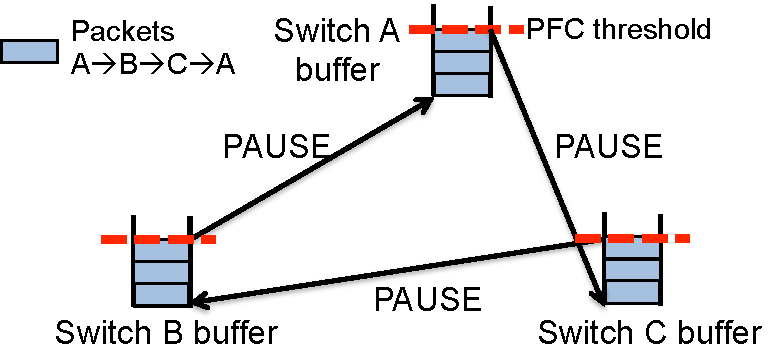
\includegraphics[width=0.45\textwidth] {figs/deadlock}
		\vspace{-1em}
		\caption{A simple (but contrived) example to illustrate CBD formation
		without routing loop.}
		\vspace{-1em}
		\label{fig:basic_deadlock}
\end{figure}

\section{Deadlock case study}\label{sec:casestudy}

In this part, we present our simulation study about three deadlock cases, and demonstrate that 1) cyclic buffer dependency is not a sufficient and necessary condition for deadlock; 2) simultaneous cyclic pause is not sufficient to create a permanent deadlock.

\begin{figure*}[t]
%\vspace{-0.1in}
\centering

\subfloat[short for lof][Topology and flows.] {
    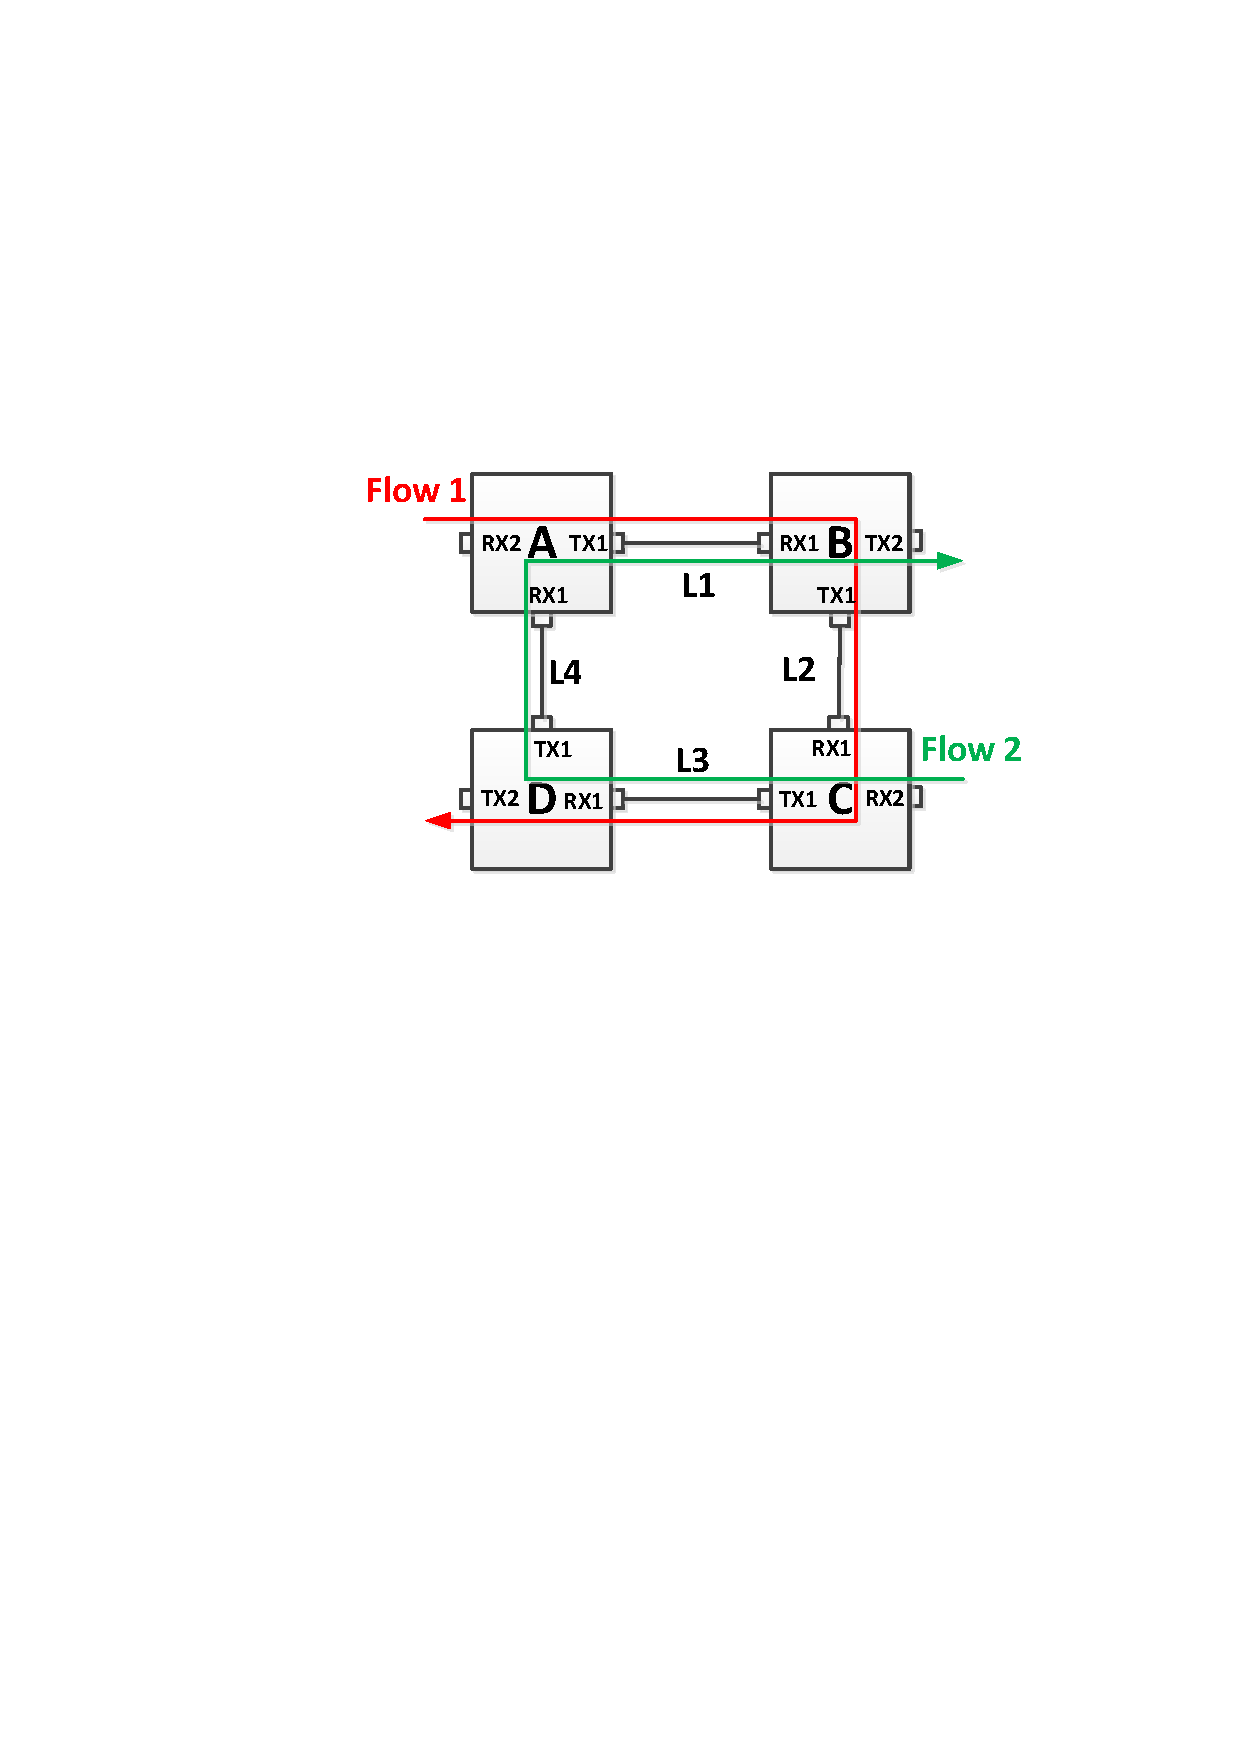
\includegraphics[width=0.35\textwidth] {figs/case1_topo.pdf}
}
\subfloat[short for lof][Buffer dependency graph.]{
    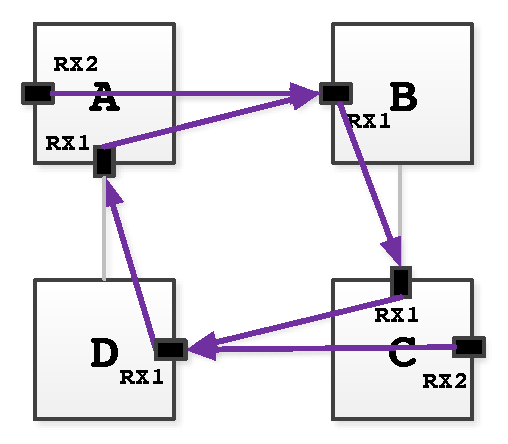
\includegraphics[width=0.24\textwidth] {figs/case1_buffer_dependency.pdf}
}
\subfloat[short for lof][Pause events at four links.]{
    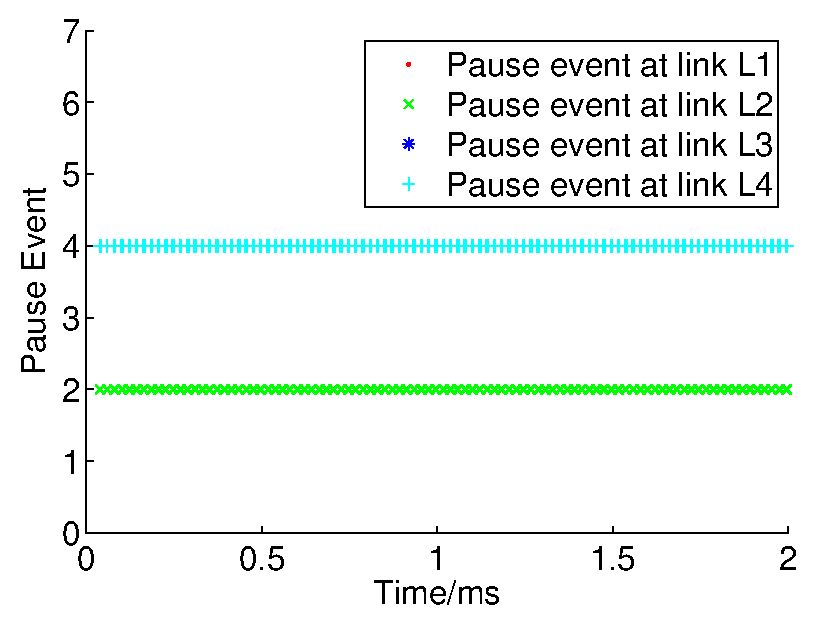
\includegraphics[width=0.3\textwidth] {figs/case1_pause.eps}
}

\subfloat[short for lof][Buffer occupancy at switch A.] {
    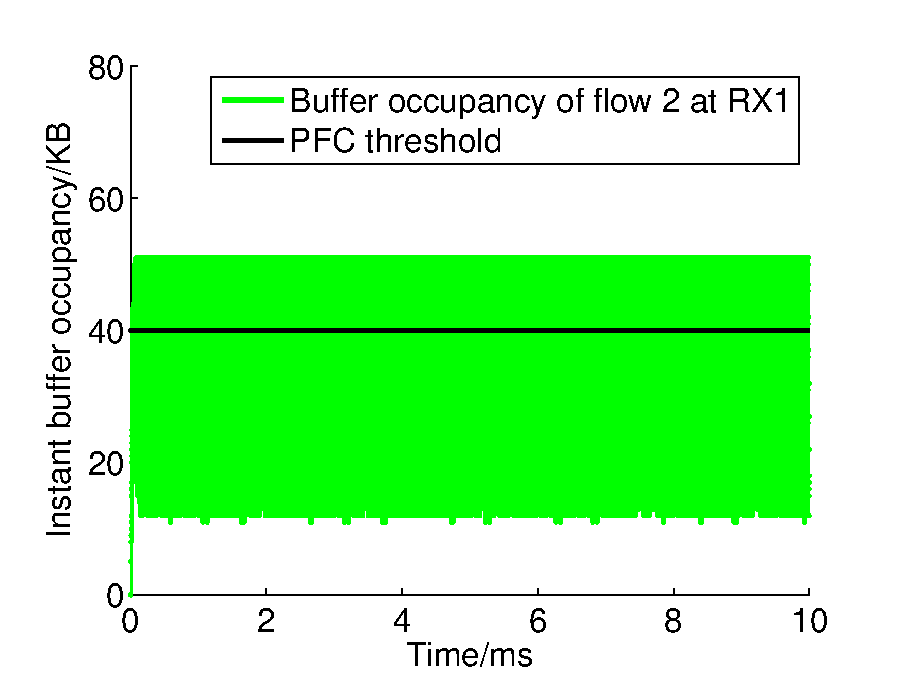
\includegraphics[width=0.25\textwidth] {figs/case1_buffer_occupancy_A.eps}
}
\subfloat[short for lof][Buffer occupancy at switch B.] {
    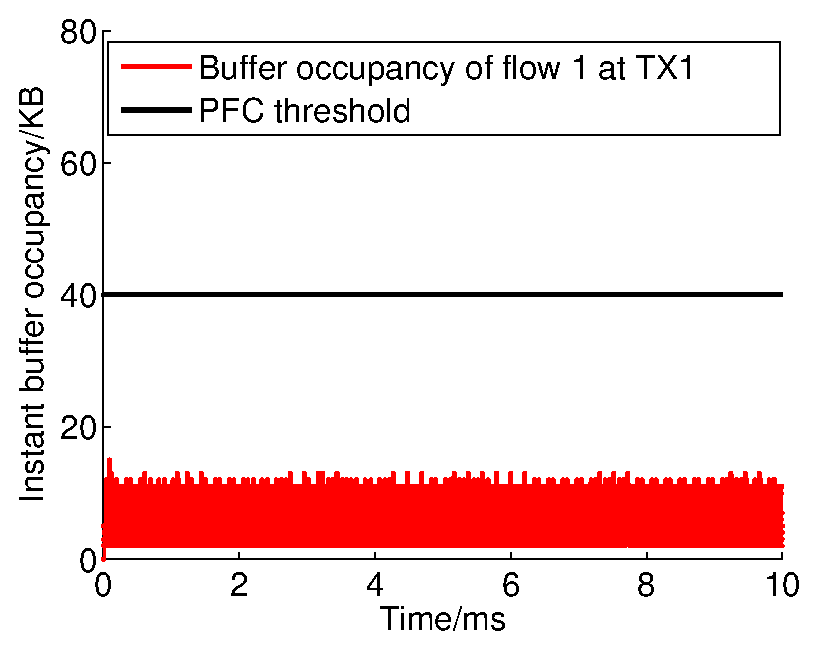
\includegraphics[width=0.25\textwidth] {figs/case1_buffer_occupancy_B.eps}
}
\subfloat[short for lof][Buffer occupancy at switch C.] {
    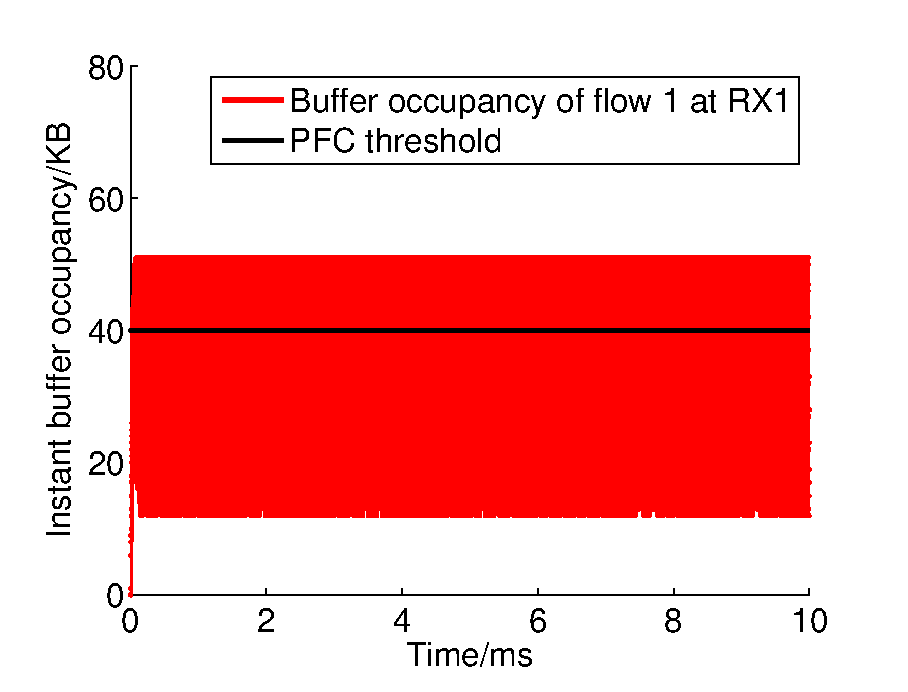
\includegraphics[width=0.25\textwidth] {figs/case1_buffer_occupancy_C.eps}
}
\subfloat[short for lof][Buffer occupancy at switch D.] {
    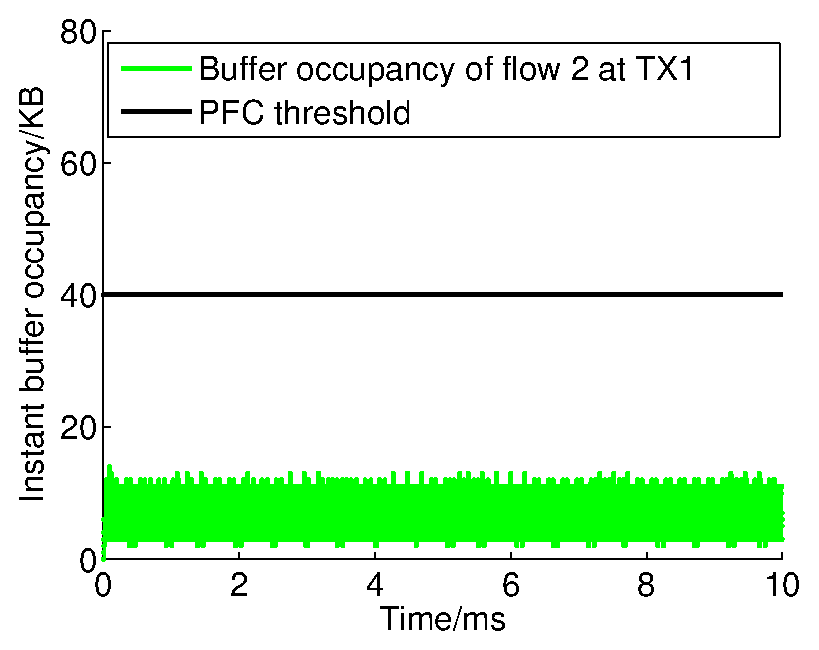
\includegraphics[width=0.25\textwidth] {figs/case1_buffer_occupancy_D.eps}
}

\caption{Deadlock case 1.}\label{fig:case1}

\end{figure*}

 \textbf{Simulation setup}: To create a well controlled experimental environment for deadlock analysis, we did our deadlock case study using packet-level NS-3 simulations. 
 
 In our modified NS-3 simulator, we implement PFC protocol (i.e., IEEE 802.1 Qbb protocol). Note that most modern commodity switches are output-queued, while PFC works in a per ingress queue fashion. Basically, for each ingress queue, the switch will maintain a counter to track its instant virtual queue length (i.e., bytes of buffered packets received by this ingress queue). Once the queue length of an ingress queue exceeds the pre-configured PFC threshold, a pause frame will be sent to the corresponding upstream device. The upstream device then stop sending any packet to this ingress queue unless 1) the pause frame has expired; 2) or it has received a resume frame from this ingress queue.
 
 In our simulations, link capacity of all links is 40Gbps. All the switches have 12MB buffer. PFC threshold is statically set to 40KB for each ingress queue.


\begin{figure*}[t]
%\vspace{-0.1in}
\centering

\subfloat[short for lof][Topology and flows.] {
    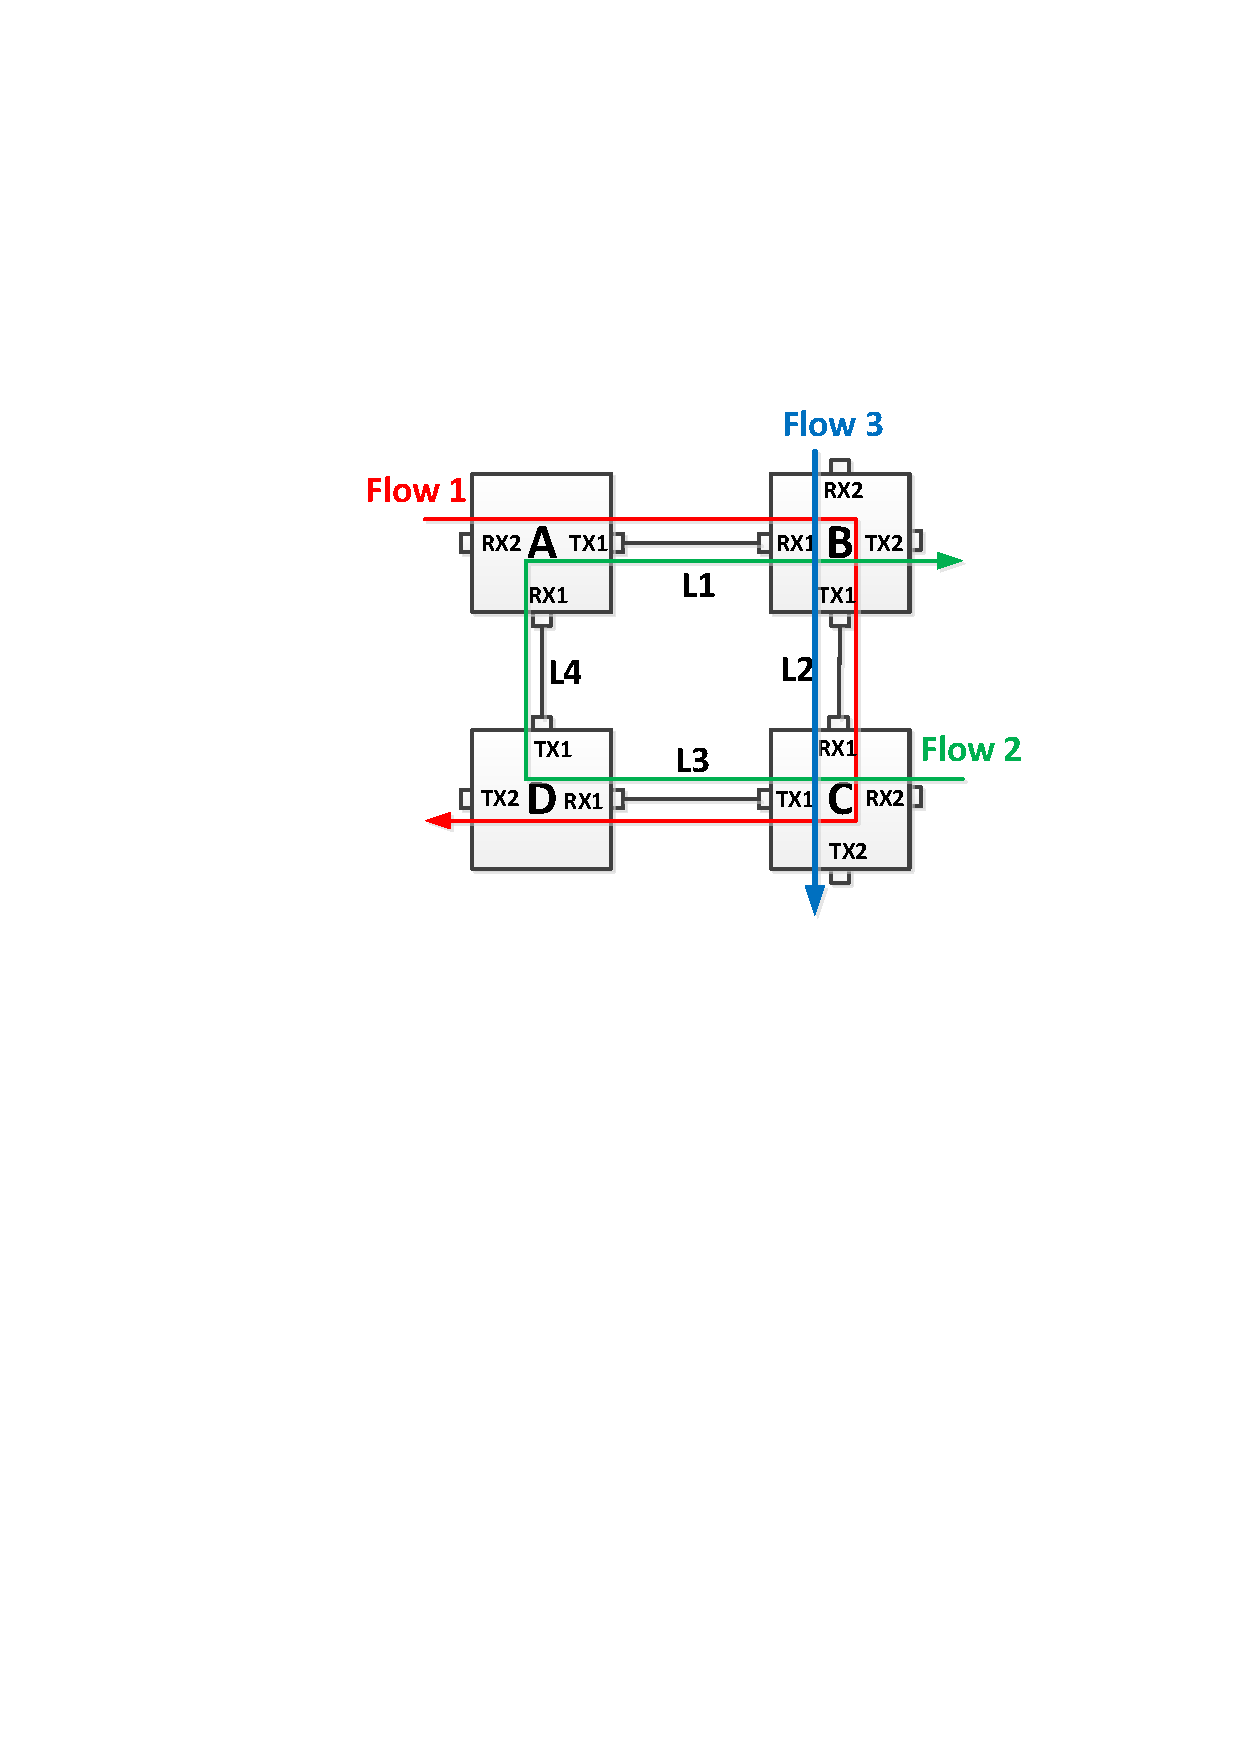
\includegraphics[width=0.37\textwidth] {figs/case2_topo}
}
\subfloat[short for lof][Buffer dependency graph.]{
    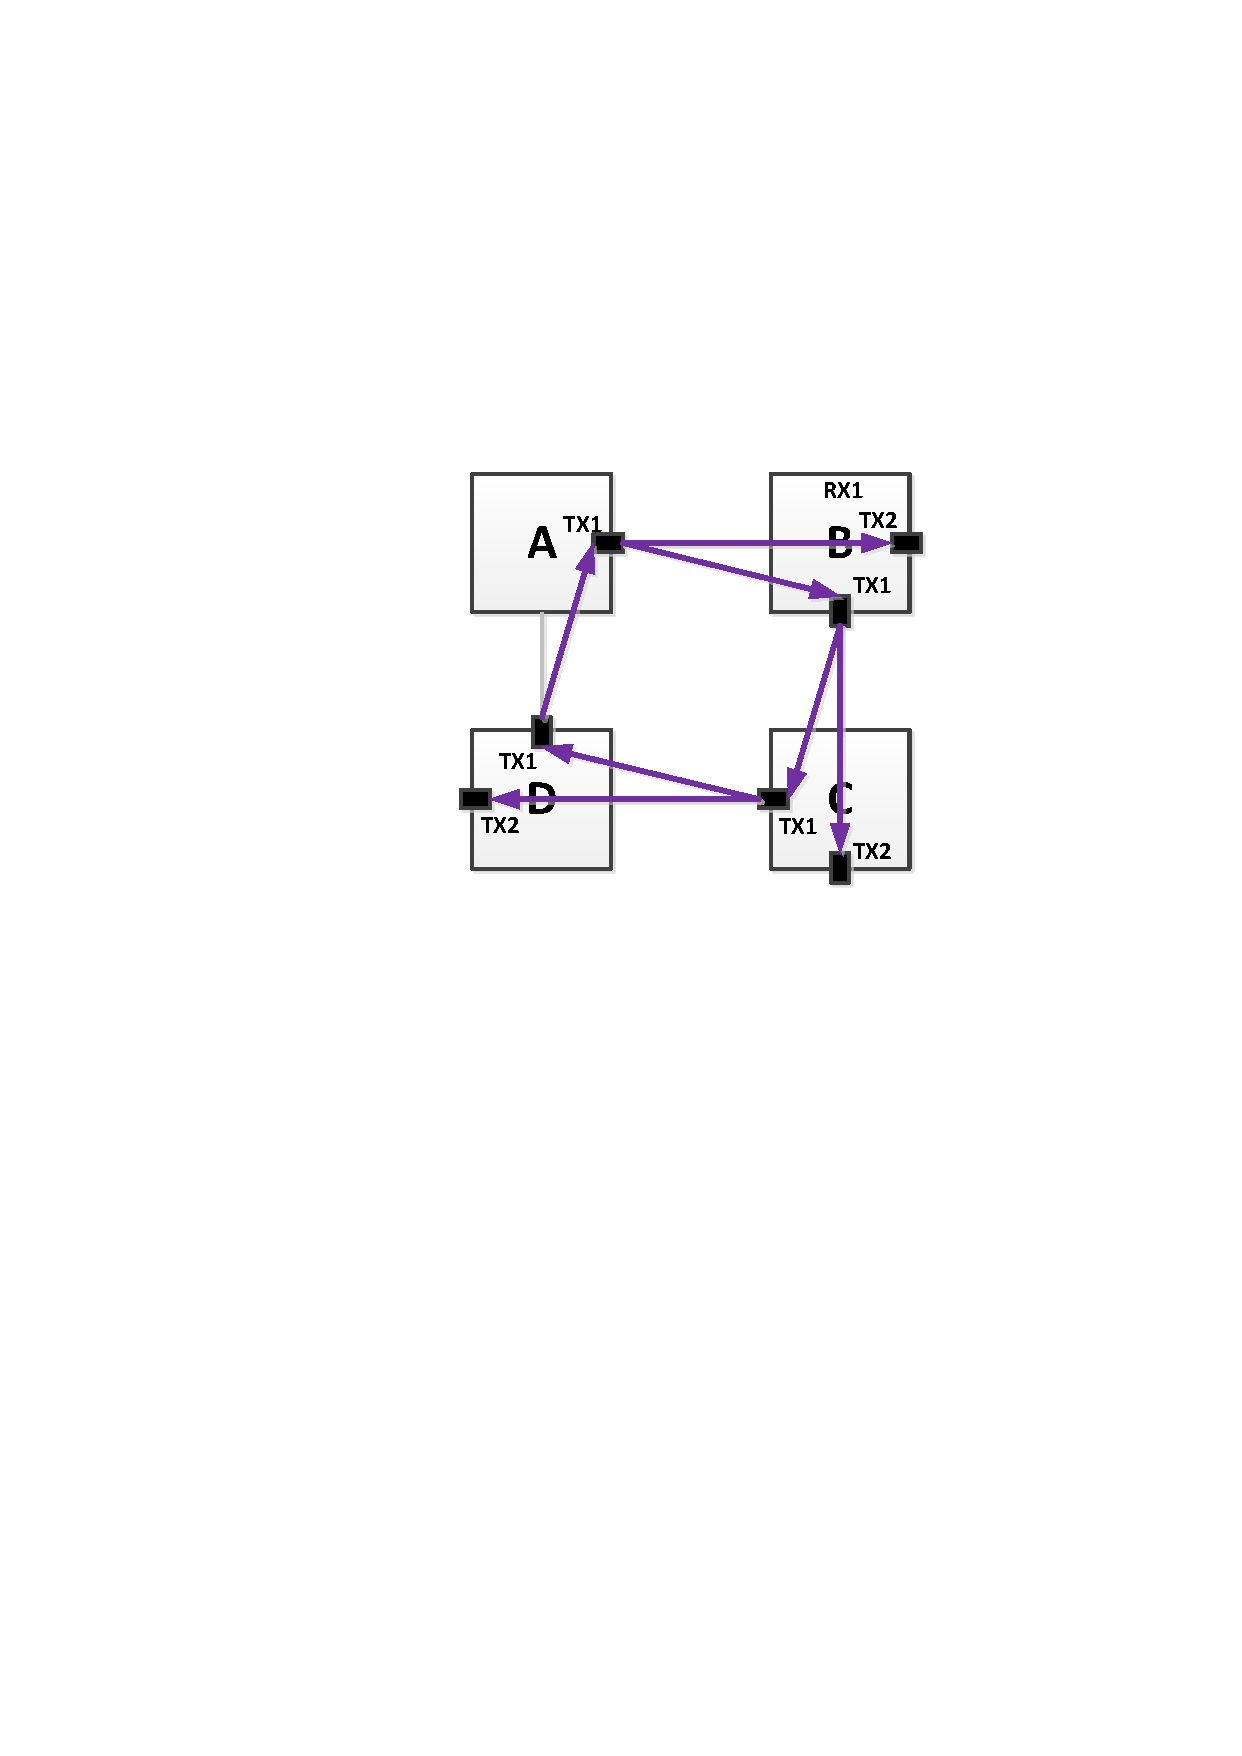
\includegraphics[width=0.27\textwidth] {figs/case2_buffer_dependency}
}
\subfloat[short for lof][Pause events at four links.]{
    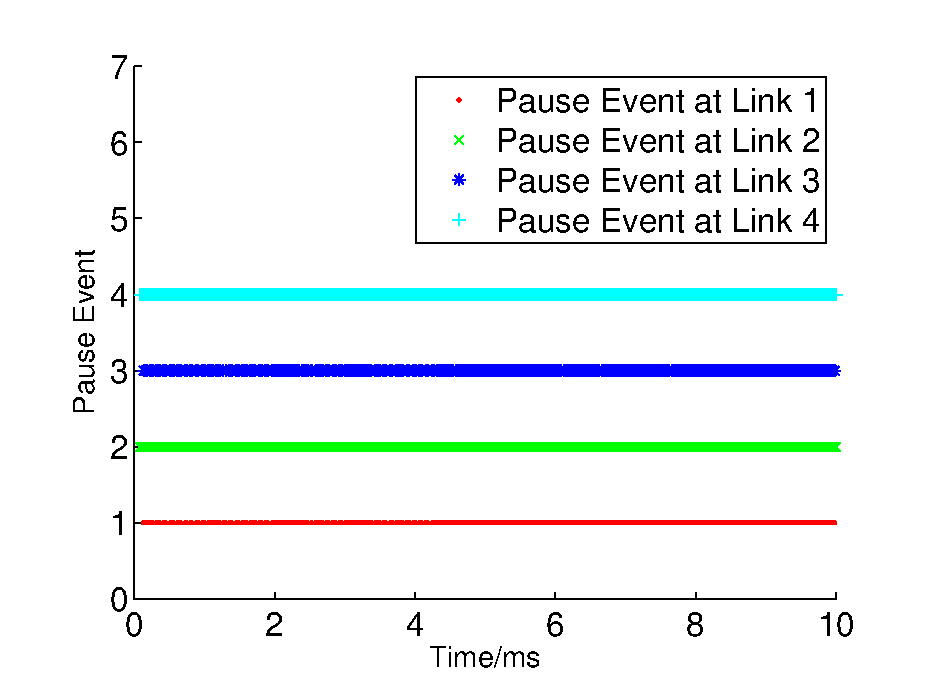
\includegraphics[width=0.3\textwidth] {figs/case2_pause.eps}
}


\caption{Deadlock case 2.}\label{fig:case2}

\end{figure*}

\textbf{Case 1:} In this case, as shown in Fig.~\ref{fig:case1}(a), we let two flows run over four switches A, B, C and D. Flow 1 starts at a host (not shown) attached to A, passes through B and C, and ends at a host attached to D. Flow 2 starts at a host attached to C, passes through D and A, and ends at a host attached to B. In the figure, RX represents input queue (or port), while TX represents output queue (or port). To evaluate whether there will be deadlock in the worst case, both flows are UDP flows with infinite traffic demand.

Buffer dependency graph of case 1 is drawn in Fig.~\ref{fig:case1}(b). Each directed line represents a buffer dependency from the source TX to the destination TX. For example, packets buffered in TX1 of A will be sent to either TX1 or TX2 of B, so in Fig.~\ref{fig:case1}(b), two directed lines are drawn there between A and B. Similarly, we can draw the dependency lines between other switches. As we can see in Fig.~\ref{fig:case1}(b), there is a cyclic buffer dependency among the four switches, i.e., dependencies from TX1 of A to TX1 of B, then to TX1 of C, then to TX1 of D, and finally back to TX1 of A.

In Fig.~\ref{fig:case1}(c), we plot the PFC pause events at four links L1, L2, L3 and L4. Basically, if link Li (i=1,2,3,4) is paused at time t, we plot a point at location (t, i). Pause events at different links are plotted with different colors and of different heights. As we can observe, links L2 and L4 are paused continuously, while the other two links L1 and L3 never get paused. In this case, deadlock will never occur as no packet will be paused permanently.

To understand the pause pattern in Fig.~\ref{fig:case1}(c), we sample the instant buffer occupancy of both flows at TX1 queues of A, B, C and D every 1us. In Fig.~\ref{fig:case1}(d), we draw the instant buffer occupancy of flow 2 at TX1 of A. Buffer occupancy of flow 1 is not drawn in Fig.~\ref{fig:case1}(d) as it does not contribute to the pause of link L1 (Note that PFC works in a per ingress queue fashion). 

Similarly, in Fig.~\ref{fig:case1}(e), Fig.~\ref{fig:case1}(f) and Fig.~\ref{fig:case1}(g), we draw the instant buffer occupancy of interested flows at TX1 queues of B, C and D, respectively. As flow 1 and flow 2 are symmetric, we only present the analysis for Fig.~\ref{fig:case1}(d) and Fig.~\ref{fig:case1}(e) to show why Link L4 is paused continuously but link L1 never gets paused.

As shown in Fig.~\ref{fig:case1}(d), buffer occupancy of flow 2 at TX1 of A fluctuates between 10KB and 55KB around the PFC threshold, so link L4 will get paused intermittently. In contrast, buffer occupancy of flow 1 at TX1 of B is well below the PFC threshold (fluctuates between 0KB and 18KB), hence link L1 will never be paused.

%In Fig.~\ref{fig:case1}(a), packets of flow 1 and flow 2 will build up at TX1 of A as both flows are competing for the capacity of link L1. Once the buffer occupancy of flow 2 exceeds the PFC threshold, RX1 of A will generate a pause frame to TX1 of D to stop packet transmission over link L4.
%
%After link L4 is paused, buffer occupancy of flow 2 will decrease as no more packets can be received by RX1 of A. Once the buffer occupancy of flow 2 is below the PFC threshold at switch A, link L4 will be resumed. Then buffer occupancy of flow 2 will start to increase again. This is why in
%
%Since packets of flow 1 buffered in TX1 of B can get transmitted at full link speed when link L2 is not paused, TX1 queue of B can not easily build up. As we can see in Fig.~\ref{fig:case1}(e), buffer occupancy of flow 1 at TX1 of B fluctuates between 0KB and 18KB, which . Hence as we can see in Fig.~\ref{fig:case1}(c), link L1 is never paused by RX1 of C.


\textbf{Observation 1:} Deadlock may not occur when cyclic buffer dependency exists in the network. Cyclic buffer dependency is just a necessary condition for deadlock.



\textbf{Case 2:} as shown in Fig.~\ref{fig:case2}(a), in the second case, in addition to case 1, we add another flow (flow 3) to run over switches B and C in sequence. All the three flows are UDP flows with infinite traffic demand. Buffer dependency graph of case 2 is drawn in Fig.~\ref{fig:case2}(b). Compared with case 1, one additional dependency from TX1 of B to TX1 of C is added.

Pause events at four links L1, L2, L3 and L4 are plotted In Fig.~\ref{fig:case2}(c). As we can see, in this case four links are all paused. To check whether deadlock will occur in this case, we stop the three flows after a sufficient long period (1000ms). What we find is that, pause events are continuously generated at all the four links even after three flows stop sending new packets (not shown in the figure). This means that a deadlock has been created among switches A, B, C and D.

In the next, we will explain why deadlock can be created by adding one additional flow to the network. After adding flow 3, packets of flow 1 buffered in TX1 of B can no longer get transmitted at full link speed due to the contention with packets of flow 3. Packets of flow 1 will then build up at TX1 of B. Once the packets of flow 1 buffered at TX1 of B exceed the PFC threshold, RX1 of B will send a pause frame to TX1 of A to pause Link L1. The pause on link L1 will help packets to build up at TX1 of A, and has a cascade effect on link L4. Due to the pause at link L1, link L4 will get paused more frequently. Then packets of flow 2 are easier to build up at TX1 of D. Once the PFC threshold is triggered at D, link L3 also get paused. So in case 2, pause events can occur at all the four links.

Once all the four links are paused simultaneously, there is a chance that no link can get resumed. For example, it is possible that when simultaneous pause happens, at switch A and switch B, the first packet buffered in the head of TX1 is a packet of flow 1, and meanwhile, at switch C and switch D, the first packet buffered in the head of TX1 is a packet of flow 2. If the above condition occurs, no link can get resumed as all the TX1 queues are waiting for its downstream neighbors to release some buffer to break the standstill condition.

\textbf{Observation 2:} Deadlock will occur when all the links in a cycle are paused simultaneously and no link can get resumed.


\begin{figure*}[t]
%\vspace{-0.1in}
\centering

\subfloat[short for lof][Topology and flows.] {
    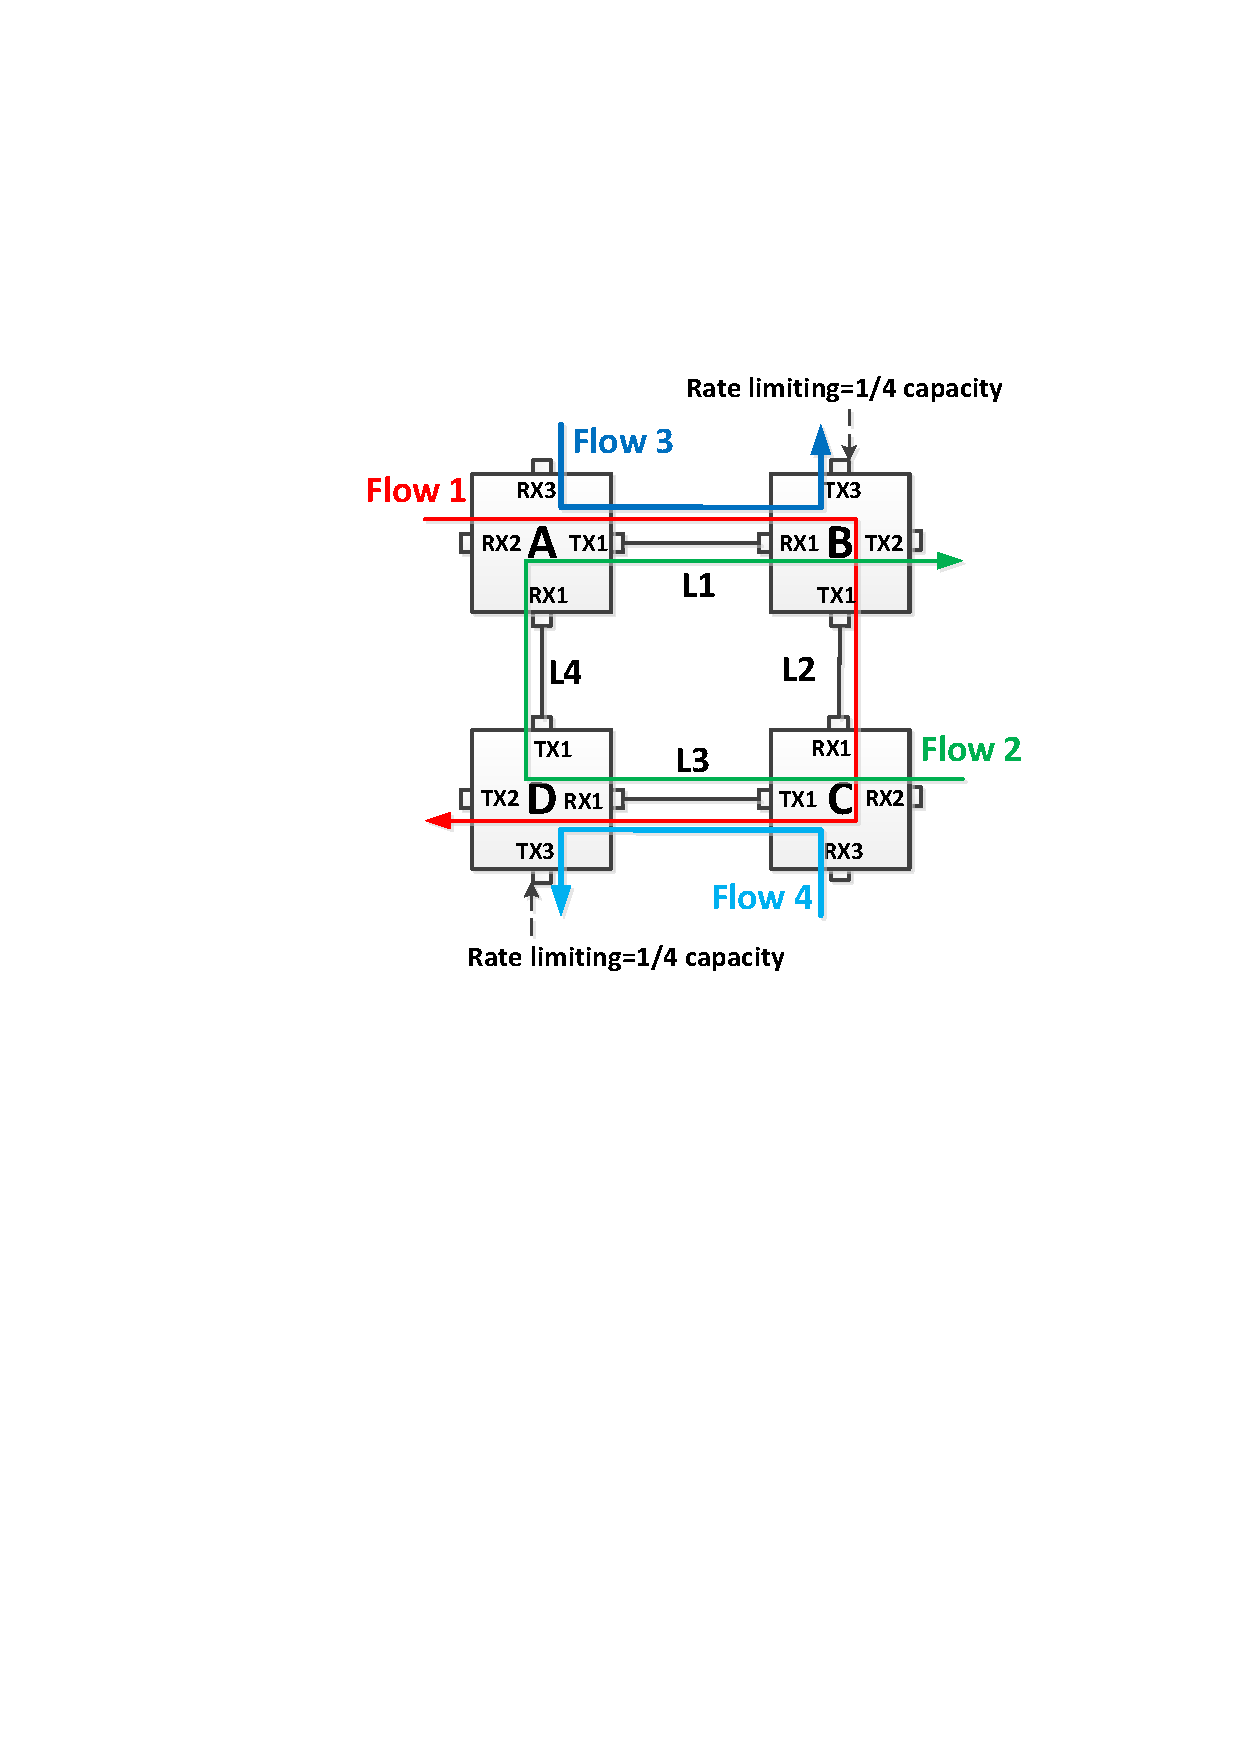
\includegraphics[width=0.37\textwidth] {figs/case3_topo}
}
\subfloat[short for lof][Buffer dependency.]{
    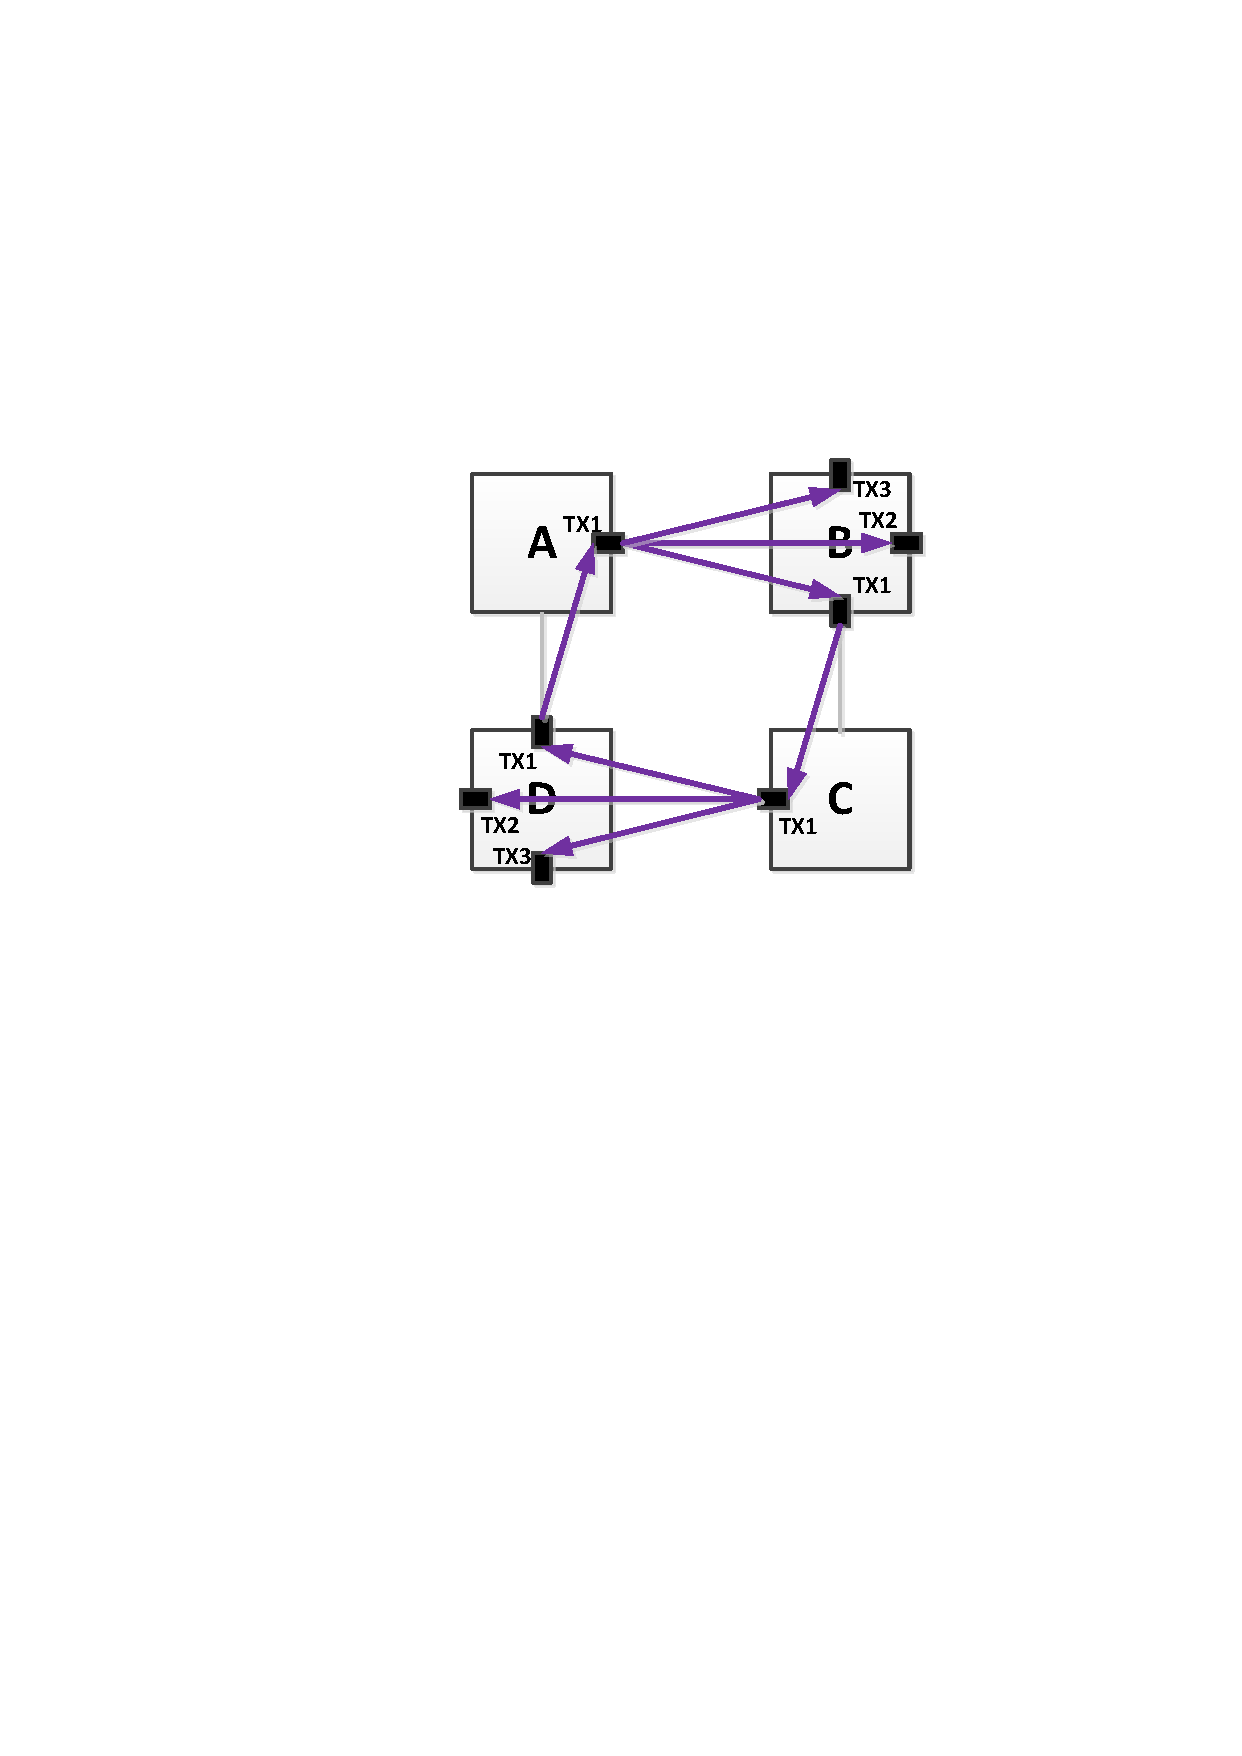
\includegraphics[width=0.28\textwidth] {figs/case3_buffer_dependency}
}
\subfloat[short for lof][Pause events at four links.]{
    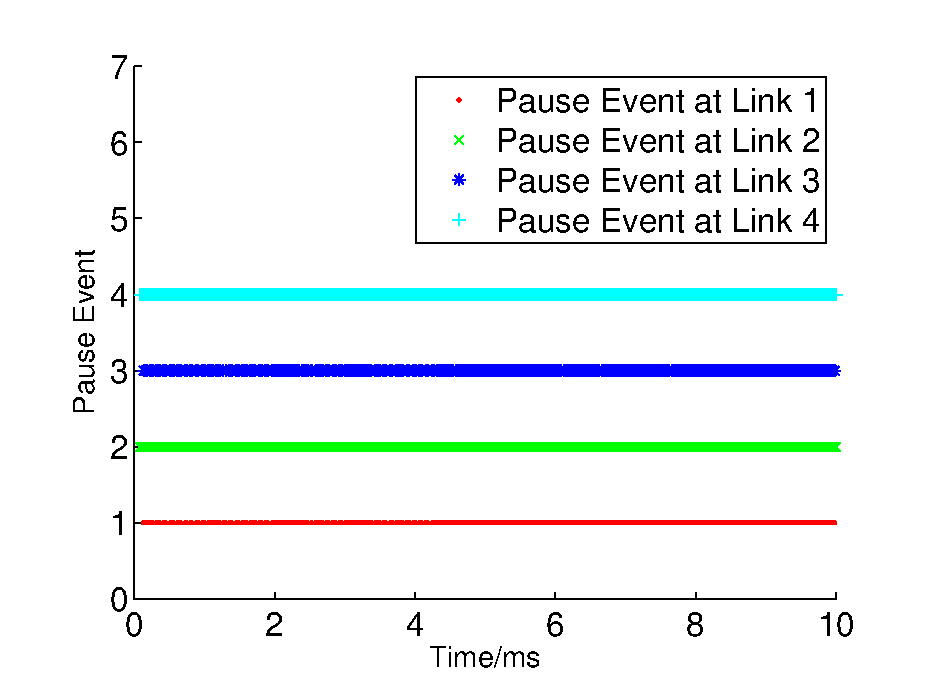
\includegraphics[width=0.3\textwidth] {figs/case3_pause.eps}
}

\subfloat[short for lof][Buffer occupancy of flow 2 at switch A.] {
    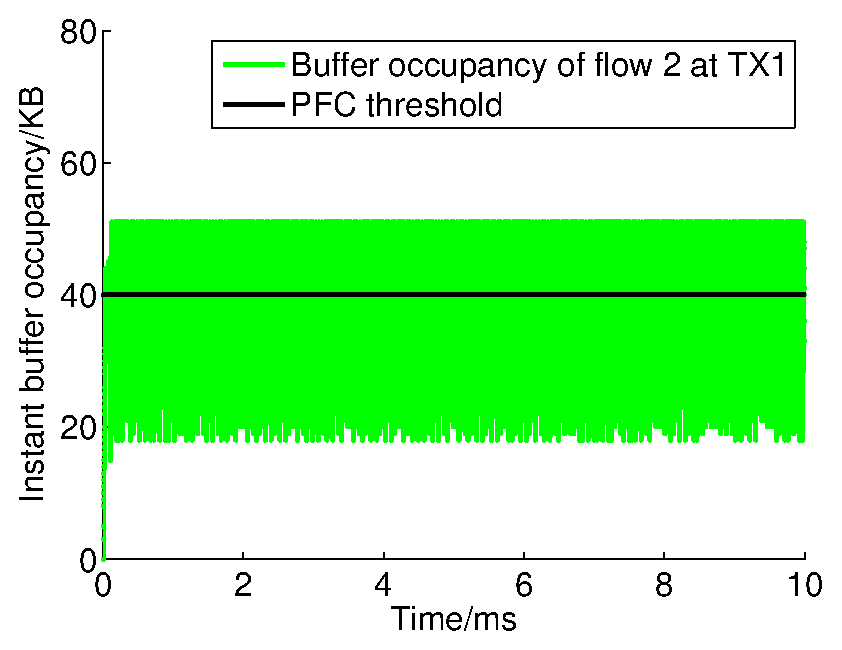
\includegraphics[width=0.33\textwidth] {figs/case3_buffer_occupancy_A.eps}
}
\subfloat[short for lof][Buffer occupancy of flow 1 at switch B.] {
    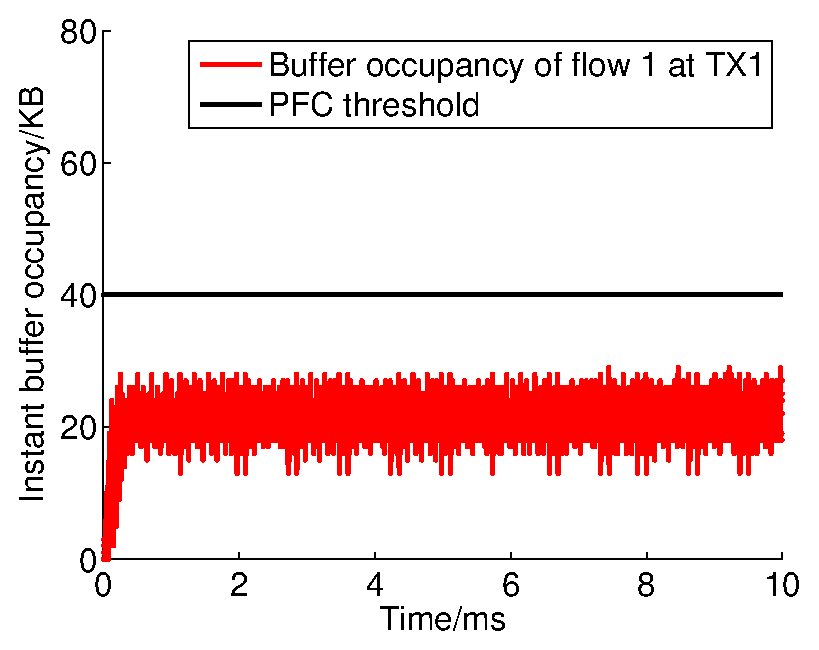
\includegraphics[width=0.33\textwidth] {figs/case3_buffer_occupancy_B1.eps}
}
\subfloat[short for lof][Buffer occupancy of flow 3 at switch B.] {
    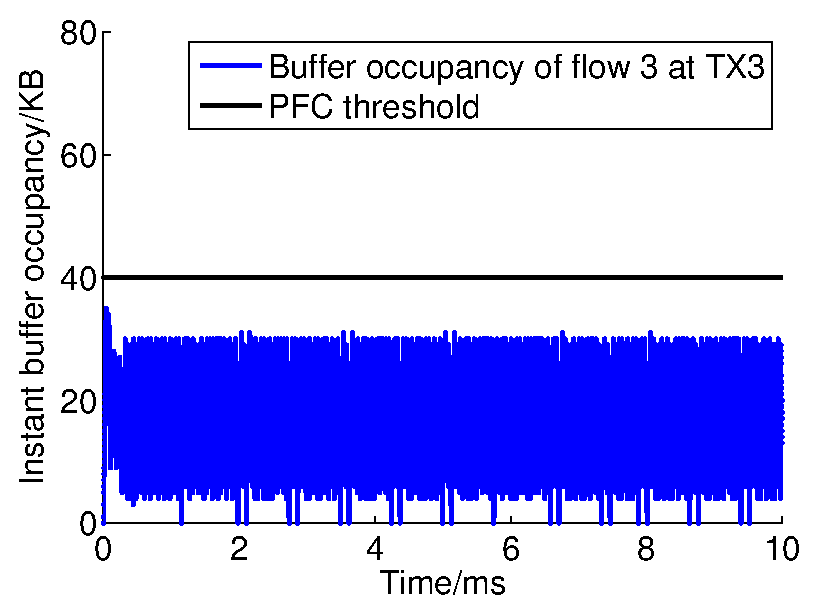
\includegraphics[width=0.33\textwidth] {figs/case3_buffer_occupancy_B3.eps}
}

\caption{Deadlock case 3.}\label{fig:case3}

\end{figure*}

\textbf{Case 3:} In this case, we will show that even if all the four links are paused simultaneously, it is not guaranteed that a deadlock will be created. As shown in Fig.~\ref{fig:case3}(a), in addition to case 1, we add another two flows (flow 3 and flow 4). Flow 3 starts at a host attached to A, passes through A and B, and ends at a host attached to B. Flow 4 is a symmetric flow of flow 3 that runs over C and D. All the four flows are UDP flows with infinite traffic demand. Two rate limiters are added at TX3 queues of B and D to ensure that rates of flow 3 and flow 4 will not exceed $1/4$ of the link capacity. Buffer dependency graph of case 3 is drawn in Fig.~\ref{fig:case3}(b). Compared with case 1, two additional buffer dependencies from TX1 queues to TX3 queues are added.

Pause events at four links L1, L2, L3 and L4 are plotted In Fig.~\ref{fig:case3}(c).  As we can see from the figure, all the four links are paused continuously. However, we find that once we stop the flows, all the links get resumed and buffer occupancy of four switches soon becomes zero. This indicates that deadlock cannot be created in case 3.

To find out why there is no deadlock in case 3, we draw the instant buffer occupancy of 3 flows at switches A and B in Fig.~\ref{fig:case3}(d), Fig.~\ref{fig:case3}(e) and Fig.~\ref{fig:case3}(f). Here we omit the buffer occupancy condition of switches C and D as the topology and the flows are symmetric.

As shown in Fig.~\ref{fig:case3}(d), at TX1 of A, the buffer occupancy of flow 2 exceeds the PFC threshold, so link L4 will get paused. To understand why link L1 is also paused, we need to consider the buffer occupancy of flow 1 and flow 3 at switch B. The reason is that packets received by RX1 of B are possible to be queued at both TX1 and TX3 (note that there is a rate limiter on TX3). As long as the sum of the buffer occupancies of both TX queues exceeds the PFC threshold, link L1 will get paused. As we can see in Fig.~\ref{fig:case3}(e) and Fig.~\ref{fig:case3}(f), although individually buffer occupancy of either TX1 or TX3 is less than the PFC threshold, their sum is larger than the PFC threshold. Hence link L1 is paused.

As both TX1 and TX3 contribute to the pause on link L1, to create a deadlock, we need to ensure that packets buffered at both TX queues cannot get resumed. However, packets buffered at TX3 can always get transmitted within a finite time as it is not involved in any cyclic buffer dependency. This explains why when we stop the flows, all the four links can be resumed from the pauses. 


\textbf{Observation 3:} even if all the links in a cycle are paused simultaneously, it is not sufficient to create a permanent deadlock.

%\subsection{Deadlock problem in RDMA DCNs}\label{subsec:deadlock_problem}
%
%Once a loop occurs in a network, packets of some flows will be caught in the loop and traverse the same links multiple times until they are dropped due to Time-to-Live (TTL) expiration. Apart from causing packet drops, loops will also waste some link bandwidth as well as increase the end-to-end delay for the flows traversing some link(s) in the loop (but not caught by the loop).
%
%\begin{figure}[t]
%\centering
%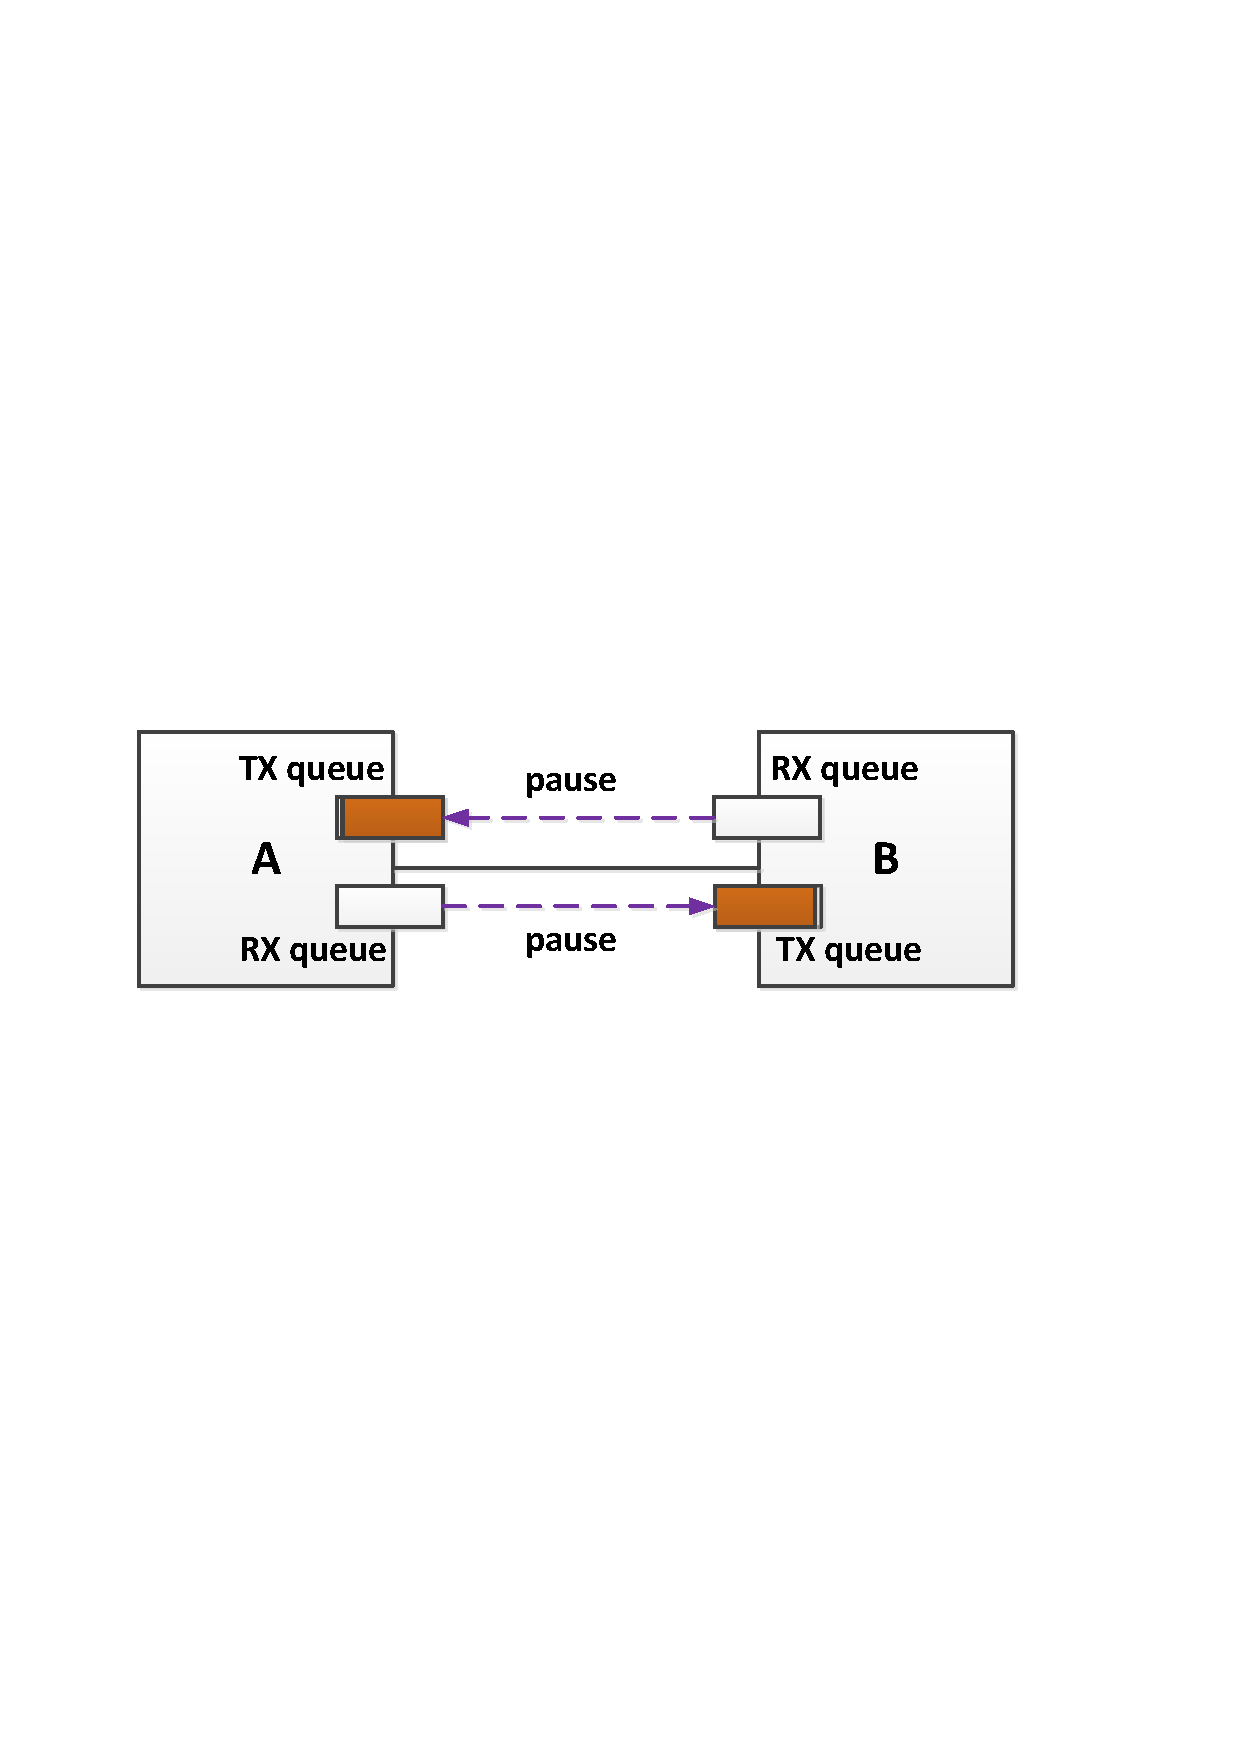
\includegraphics[width=0.45\textwidth,center]{figs/deadlock_example.pdf}
%\caption[Optional caption for list of figures]{An example of loop induced deadlock: there is a loop between switch A and switch B. Both TX queues (egress queues) are paused by PFC as no buffer are available at both switches to accommodate more packets.}
%\label{fig:loop_deadlock}
%\end{figure}
%
%In a lossy network, the impact of a loop is not fatal and can be completely eliminated as long as the loop is removed from the network. In contrast, in a lossless network, if packets enter a loop faster than they get dropped in the loop due to TTL expiration, packets will occupy the buffer of all the switches in the loop, and then a deadlock is created. When a deadlock occurs, each switch in the loop is paused by its downstream switch, and at the same time pauses its upstream switch due to the lack of available buffer to accept more packets. Once such a circular buffer dependency is created, the deadlock condition will hold persistently even after the loop is eliminated.
%
% Under deadlock condition, no packets can move along the links in the loop, and more and more devices outside the loop will be paused due to the cascade effect of PFC. If a deadlock is created in the core of the network, it is very likely to bring the whole data center into a deadlock state.
%
%A simple deadlock example is shown in Fig.~\ref{fig:loop_deadlock}. In this example, there is a routing loop between switch A and switch B. Packets enter this loop at a sufficient large rate and soon occupy all the available buffer of both switches. Then Both TX queues (egress queues) will be paused by PFC PAUSE frames and a deadlock is created. As we can see, this deadlock cannot be resolved by eliminating the routing loop as packets are already queued in the TX queues and can never reach the next-hop switch to escape from the loop.
%
%\subsection{Sufficient condition for deadlock creation}\label{subsec:deadlock_condition}
%
%In this part, we analyze the sufficient condition to create a deadlock when there is a loop in the network.
%
%At first, we consider the maximum packet drain rate in a loop regarding TTL expiration. Let $n$ the number of switches in a loop, $B$ be the link bandwidth and $k_{TTL}$ be the TTL value of packets before they enter the loop. Each time a packet traverses one switch, its TTL value will be reduced by 1.
%
%The maximum packet drain rate is achieved when no switch is paused by PFC PAUSE frame and each switch is sending packets to its next-hop in the loop at the rate of $B$. So the maximum packet drain rate $r^{max}_d$ is equal to $nB/k_{TTL}$. here $nB$ can be viewed as the maximum packet ``flowing" rate in the loop, while $1/k_{TTL}$ captures the information that a packet will be dropped after it has traversed $k_{TTL}$ hops of switches in the loop.
%
%Let $r_{in}$ be the injection rate of packets into the loop. One sufficient condition to create a deadlock in a lossless network is that: there is a loop
%in the network, and condition $r_{in} > r^{max}_d$ holds for a sufficient long period until a circular buffer dependency is created in the loop.
%
%\begin{figure}[t]
%\centering
%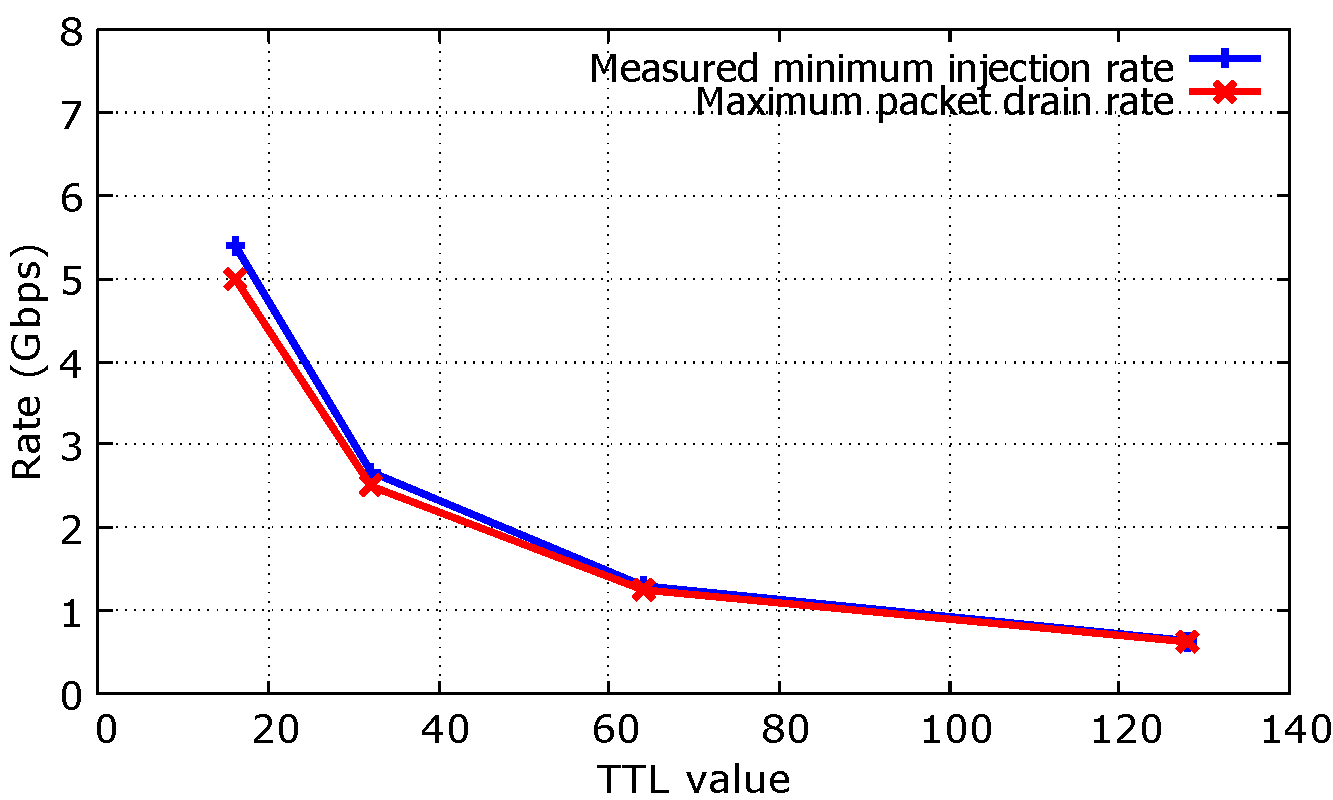
\includegraphics[width=0.5\textwidth,center]{figs/r_and_rdrain.pdf}
%\caption[Optional caption for list of figures]{Measurement of the minimum injection rate to create a deadlock. Both switches in the loop are Arista 7050QX32.}
%\label{fig:mrate_measurement}
%\end{figure}
%
%To verify our analysis above, we manually configure a loop between two 40Gbps switches, and measure the minimum packet injection rate that can create a deadlock. The result is shown in Fig.~\ref{fig:mrate_measurement}. As we can see, the measured minimum packet injection rate is just slightly larger than the maximum packet drain rate which is computed according to $nB/k_{TTL}$. This observation holds when TTL is set to different values.
%
%Another observation from the figure is that, setting smaller TTL can help to prevent deadlock but its benefit is limited. As shown in the figure, when TTL is set to 16 which is already a very small value, the minimum injection rate is only about 6Gbps.
%
%\subsection{Analysis of the time to create a deadlock}\label{subsec:deadlock_condition}
%
%In this part, we analyze and measure the time to create a deadlock when the sufficient condition for deadlock creation is already met. Deadlock creation time is related to three factors: \textbf{packet injection rate $r_{in}$}, \textbf{packet drain rate $r_{d}$} and \textbf{PFC threshold $t_{PFC}$}.
%
%$t_{PFC}$ determines the minimum bytes of packets needed to be ``trapped" in the loop to create a deadlock, while $r_{in} - r_{d}$ can be viewed as the packet increase rate.
%
%%Packet injection rate is determined by the instant traffic demand of applications running in the data center. A larger injection rate requires less time to create a deadlock.
%%
%%As discussed above, the maximum packet drain rate will be a fixed value once $n$, $B$ and $k_{TTL}$ is determined. We find that packet drain rate will decrease significantly after packets are queued in the loop because it will take a packet much longer time to get dropped in the loop when there is queuing delay.
%
%Most modern commodity switches use a dynamic $\alpha$ algorithm to determine the value of PFC threshold: Let $\alpha$ be a parameter with the range from 0 to 1, $m$ be the total switch buffer size and $m^\prime$ be the amount of buffer currently occupied. For a given $\alpha$, the value of $t_{PFC}$ is dynamically computed according to the following equation $ t_{PFC} = \alpha(m - m^\prime)$. During runtime, once the queue length of an ingress queue exceeds the instant $t_{PFC}$, a PAUSE frame will be sent to its upstream device. Note that a PAUSE frame will take some time to arrive an upstream device and take effect. To avoid packet loss due to this delay, some buffer headroom must be reserved for each ingress queue, and hence the value of $m$ in the equation is usually slightly smaller than the total switch buffer size.
%
%%
%
%
% %Most modern commodity switches share memory buffer among all ports. In order to better utilize the available shared buffer in a timely fashion, instead of setting a fixed PFC threshold,
%%A PAUSE frame will take some time to arrive an upstream device and take effect. To avoid packet loss due to this propagation delay, we must reserve enough
%%buffer headroom for each ingress queue to accommodate packets a switch may receive before a PAUSE frame finally takes effect. Let $\Delta m$ be the total amount of reserved buffer headroom. The $m$ in the above equation should be modified to be $m - \Delta m$.
%%Switches and NICs will track the value of $m^\prime$ and update the value of $t_{PFC}$ during runtime.
%
%%A smaller $\alpha$ value can lead to a shorter creation time of deadlock.  This is because a smaller $\alpha$ value means a smaller PFC threshold, while a smaller PFC threshold requires less packets to trigger a switch queue to send PAUSE frames to stop its upstream neighbors.
%
%In the next, we measure the time to create a deadlock when setting different $\alpha$ and TTL values.
%
%
%\begin{figure}[t]
%\centering
%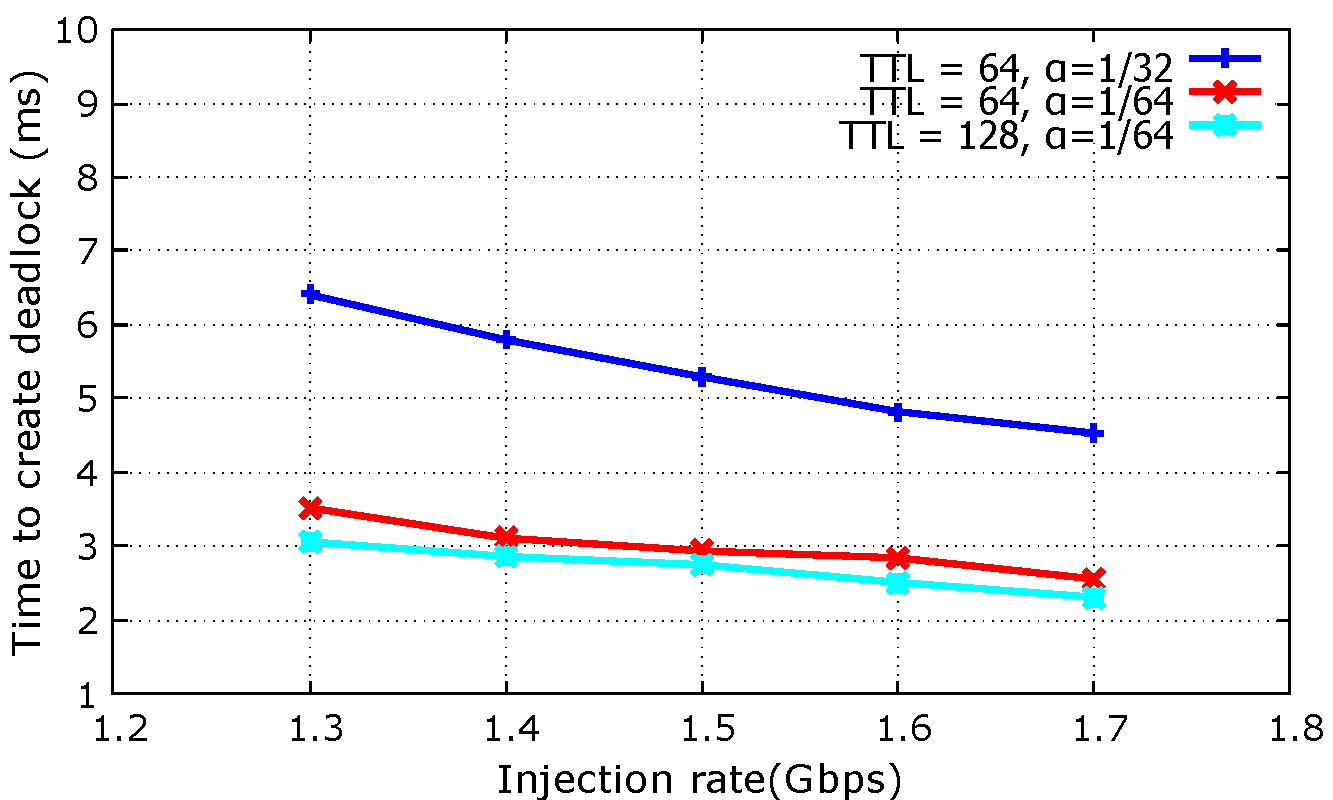
\includegraphics[width=0.5\textwidth,center]{figs/r_dltime.pdf}
%\caption[Optional caption for list of figures]{Measurement of the time to create a deadlock under different settings (deadlock will not occur when the injection rate is less than 1.3Gbps).}
%\label{fig:dltime_measurement}
%\end{figure}
%
%\parab{Measurement of the time to create a deadlock:} We manually configure a loop between two Arista 7050QX32 switches which have 32 full duplex 40Gbps ports and 12MB shared buffer. In Fig.~\ref{fig:dltime_measurement}, we set $\alpha$ and $TTL$ to different values and measure the time to create a deadlock under different injection rates.
%
%We can make four observations from the results in Fig.~\ref{fig:dltime_measurement}: 1) It takes only a few milliseconds to create a deadlock even when the injection rate is less than 2Gbps. This indicates that it is easy for a deadlock to occur even when only a transilient loop exists in the network. In addition, we cannot rely on any loop detection and recovery solutions to prevent the occurance of deadlocks as they are too slow to resolve the loop within a few milliseconds. 2) As the injection rate increases, the time to create a deadlock decreases accordingly. 3) Given a fixed injection rate, a smaller $\alpha$ value requires less time to create a deadlock. 4) Given a fixed injection rate, a smaller TTL value requires more time to create a deadlock. This is because a smaller TTL value will make the packets get dropped faster in the loop, and thus more packets are needed to be injected into the loop to trigger switch to pause each other.
%
%We repeated this experiment using many other combinations of TTL and $\alpha$ values and different number of switches. We found that all the results comply with what have been shown in Fig.~\ref{fig:dltime_measurement}.
%
%The takeaway of this experiment is that: once there is a loop in the network, deadlock is easy to occur and very hard to prevent (a deadlock can be created within a few milliseconds). In addition to a fast loop detection mechanism, we need an effective solution to detect and resolve deadlocks caused by all kinds of loops.

%\parab{Estimation of the time to create a deadlock:}

%\parab{Sufficient condition for deadlock creation:} \todo{(detailed content to be added later.)}
%
%   1. Analysis of the maximum packet drain rate caused by TTL expiration: $r^{max}_d = nB/k_ttl$.
%
%   2. Using testbed experiments to demonstrate that $r > r^{max}_d$ is a sufficient condition for deadlock creation.
%
%\parab{Creation time of deadlock:} \todo{(detailed content to be added later.)}
%
%   1. Analysis of the upper bound and lower-bound of the creation time of deadlock.
%
%   2. a) Using testbed experiments to demonstrate that lower-bound value is already a tight estimation when $r << B$; b) Analysis of the impact of PFC PAUSE frames on $r$ and $r^{max}_d$.
%
%\subsection{Analysis of device bug induced deadlock}\label{subsec:analysis_loop_deadlock}
%\todo{to be added.}

%\section{Reconfiguration-induced Deadlock}\label{sec:reconfigdeadlock}



While PFC deadlock can be avoided by leveraging a routing function that introduces no cycle in the buffer dependency graph. However, this approach cannot eliminate the cyclic buffer dependency that may arises during routing reconfiguration process.

In this part, we use examples to show 1) cyclic buffer dependency can be generated for both tree based and non-tree based DCNs when the routing reconfiguration is not well planed; 2) a bad deadlock-free reconfiguration plan will lead to a slow reconfiguration process.

\subsection{Deadlock Under Tree Based DCNs}\label{subsec:treecase}

\begin{figure}[t]
	\centering
	
	\subfloat[short for lof][Initial routing configuration.] {
		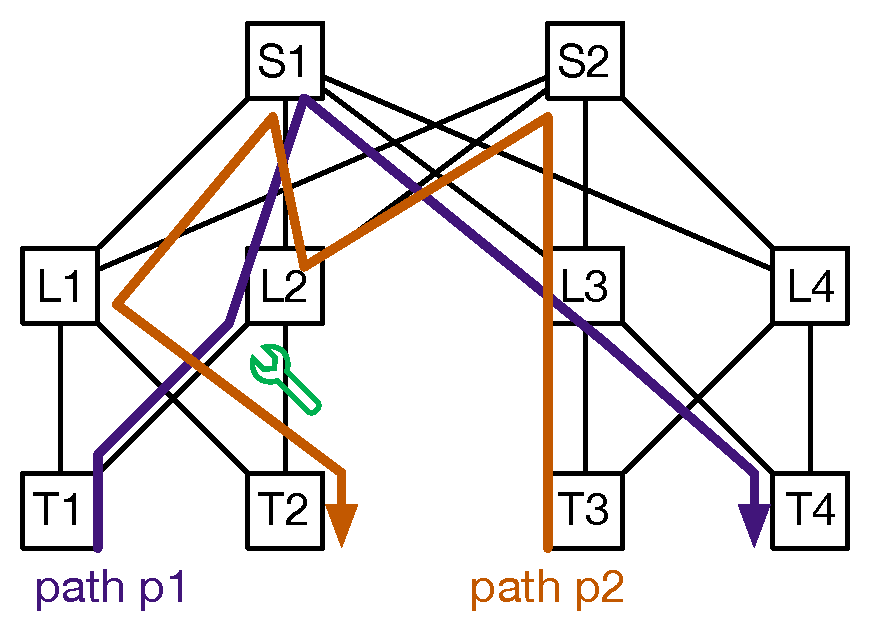
\includegraphics[width=0.24\textwidth] {figs/deadlock_tree_a}
	}
	\subfloat[short for lof][Routing configuration after reconfiguration.]{
		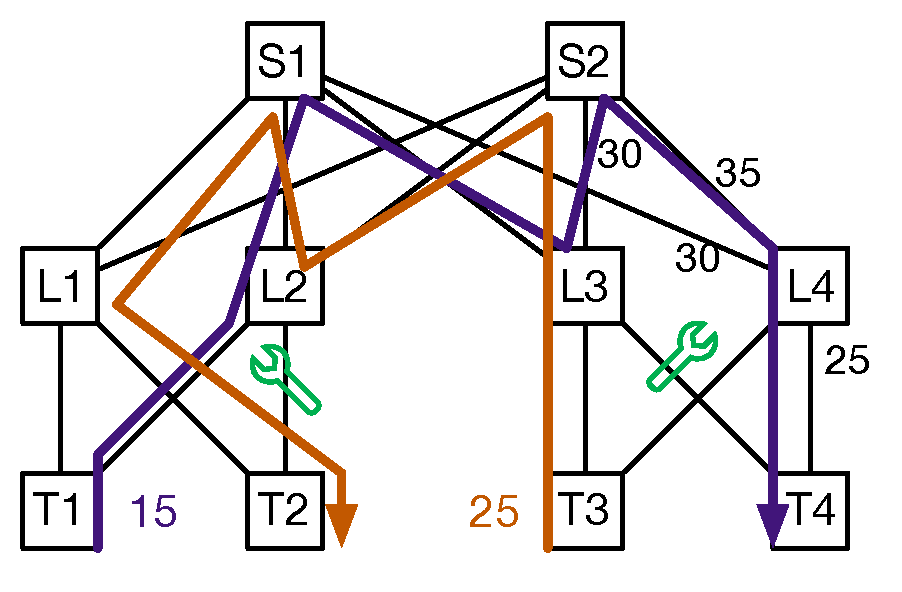
\includegraphics[width=0.24\textwidth] {figs/deadlock_tree_b}
	}
	
	\subfloat[short for lof][Intermediate routing configuration 1.] {
		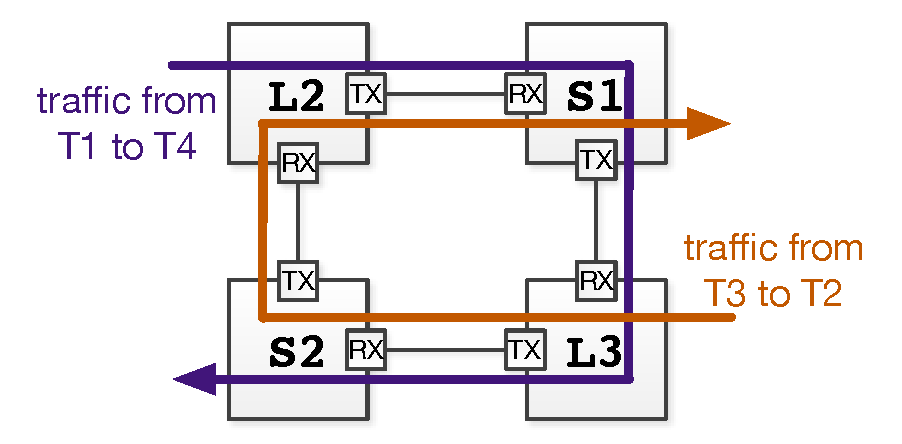
\includegraphics[width=0.24\textwidth] {figs/deadlock_tree_c}
	}
	\subfloat[short for lof][Intermediate routing configuration 2.] {
		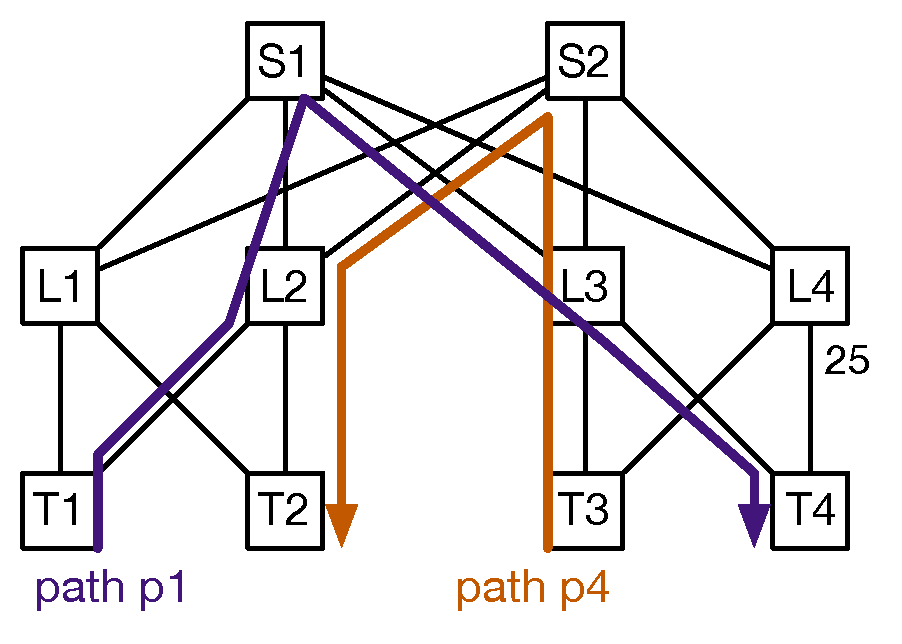
\includegraphics[width=0.24\textwidth] {figs/deadlock_tree_d}
	}
	
	\subfloat[short for lof][Buffer dependency graph.]{
		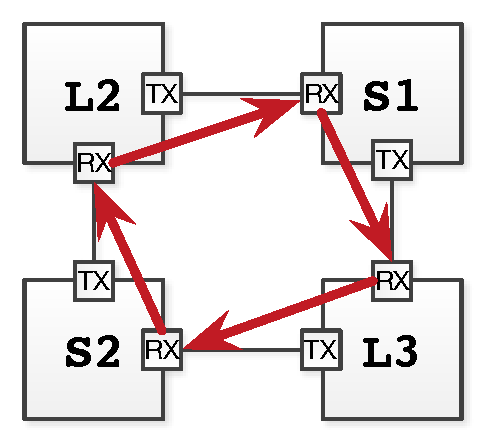
\includegraphics[width=0.2\textwidth] {figs/deadlock_tree_e}
	}
	\subfloat[short for lof][Deadlock-free reconfiguration schemes.] {
		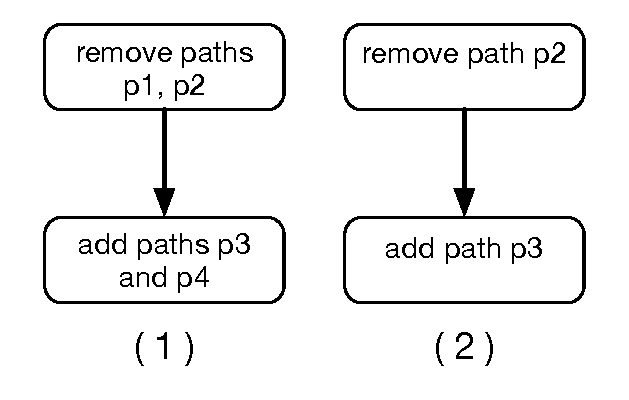
\includegraphics[width=0.28\textwidth] {figs/treecase_dfschemes}
	}
	
	\caption{Reconfiguration-induced deadlock case for tree topology.}\label{fig:treecase}
	
\end{figure}

Fig.~\ref{fig:treecase}(a) shows a small Leaf-Spine topology, which is a typical tree based DCN topology.

\textbf{Reconfiguration scenario:} For maintenance reason, the network operator now wants to replace two links L2-T2 and L3-T4 in the network. The link replacement is scheduled to be executed with two steps. The first step is to replace link L2-T2, and the second step is to replace link L3-T4.

To avoid long-term packet loss during link replacement, the network traffic passing through the operated link needs to be migrated to some other paths. 

In the first step, part of the traffic from switch T3 to switch T2 is migrated to a non-shortest path p2 because link L2-T2 is down, as shown in Fig.~\ref{fig:treecase}(a). In the second step, part of the traffic from switch T1 to switch T4 is migrated to a non-shortest path p3 because link L3-T4 is down, as shown in Fig.~\ref{fig:treecase}(b).

Let $\textbf{R}_s = \{p1, p2\}$, and $\textbf{R}_t = \{p3, p4\}$. It is easy to check both $\textbf{R}_s$ and $\textbf{R}_t$ are deadlock-free routing functions. 

\textbf{Cyclic buffer dependency during reconfiguration process:} In order to proceed from the first step to the second step, a routing reconfiguration is required to transition the routing function from $\textbf{R}_s$ to $\textbf{R}_t$.

During the reconfiguration process, different executed orders of configuration operations will lead to different intermediate routing functions. Specifically, if path p3 is added to the routing function before path p2 is removed, the intermediate routing configuration shown in Fig.~\ref{fig:nontreecase}(c) will be created. If path p4 is added to the routing function before path p1 is removed, the intermediate routing configuration shown in Fig.~\ref{fig:nontreecase}(d) will be created.  

The intermediate routing configuration shown in Fig.~\ref{fig:nontreecase}(c) introduces a cyclic buffer dependency.  To help readers understand this, in Fig.~\ref{fig:treecase}(e), we draw the buffer dependency among four switches L2, L3, S1 and S2. We reposit the locations of these four switches and draw both ingress queues (RX) and egress queues (TX) for the purpose of better explanation. As we can see, there is a cyclic buffer dependency among the ingress queues. This indicates that the network is now exposed to the danger of PFC deadlock.

\textbf{Deadlock-free reconfiguration schemes:} In Fig.~\ref{fig:nontreecase}(f), we present two possible deadlock-free reconfiguration schmes. The first scheme is to remove all the paths in $\textbf{R}_s$ before adding any new paths in $\textbf{R}_t$. This scheme will lead to a slow reconfiguration process as all the operations of adding new paths are delayed by the operations of removing old paths. 

The second scheme only requires path p2 to be removed before path p3 is added. All the other paths not mentioned can be updated freely without any order constraint. Hence the speed of routing reconfiguration can be improved.


\subsection{Deadlock Under Non-tree Based DCNs}\label{subsec:nontreecase}

\begin{figure}[t]
	\centering
	
	\subfloat[short for lof][4-node network \textbf{N}.] {
		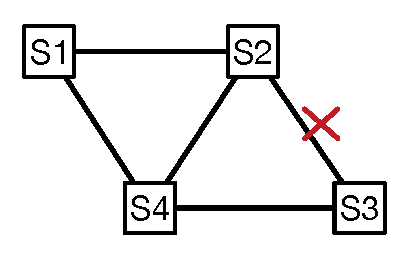
\includegraphics[width=0.16\textwidth] {figs/deadlock_nontree_a}
	}
	\subfloat[short for lof][Spanning tree \textbf{T1}.]{
		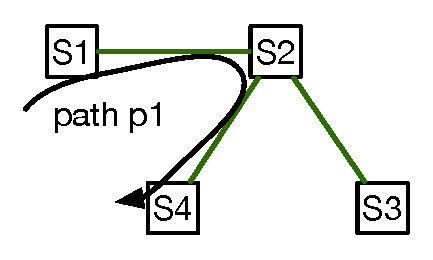
\includegraphics[width=0.16\textwidth] {figs/deadlock_nontree_b}
	}
	\subfloat[short for lof][Spanning tree \textbf{T2}.]{
		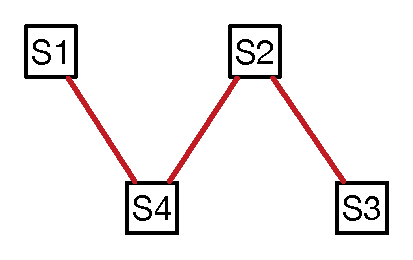
\includegraphics[width=0.16\textwidth] {figs/deadlock_nontree_c}
	}
	
	\subfloat[short for lof][Spanning tree \textbf{T3}.] {
		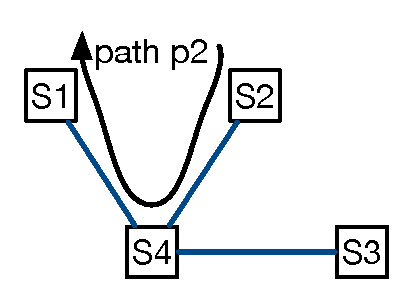
\includegraphics[width=0.16\textwidth] {figs/deadlock_nontree_d}
	}
	\subfloat[short for lof][Spanning tree \textbf{T4}.] {
		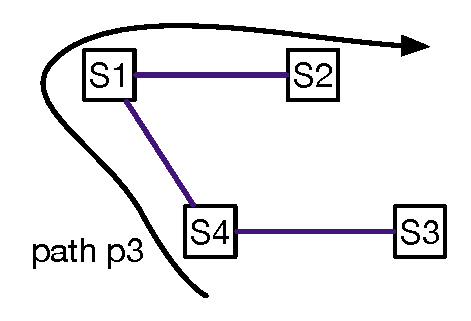
\includegraphics[width=0.16\textwidth] {figs/deadlock_nontree_e}
	}
	\subfloat[short for lof][Buffer dependency graph.]{
		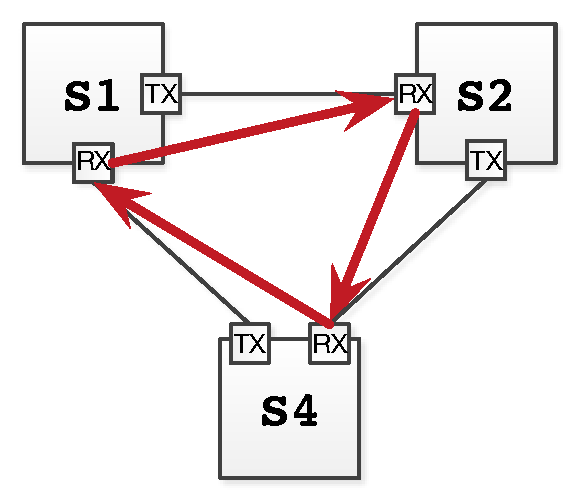
\includegraphics[width=0.15\textwidth] {figs/deadlock_nontree_f}
	}
	
	\caption{Reconfiguration-induced deadlock case for non-tree topology.}\label{fig:nontreecase}
	
\end{figure}

\begin{figure}[t]
	\centering
	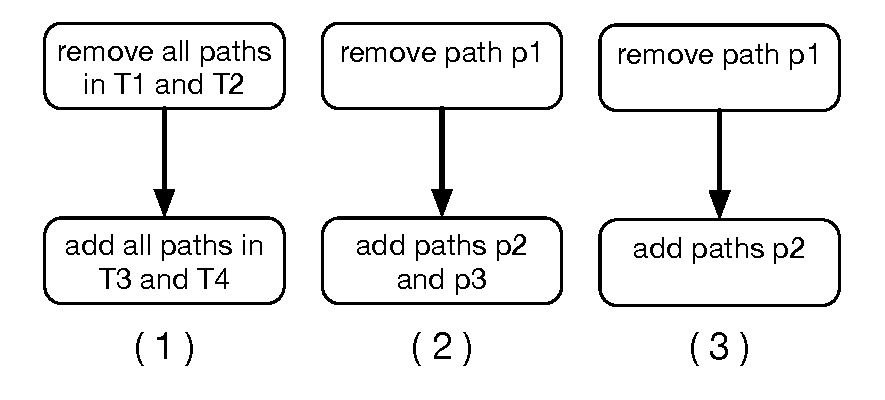
\includegraphics[width=0.45\textwidth] {figs/nontreecase_dfschemes}
	\caption{Three deadlock-free reconfiguration schemes.}\label{fig:dfschemes}
	
\end{figure}

As shown in Fig.~\ref{fig:nontreecase}(a), in this example we consider a 4-node network \textbf{N}. This topology can be a subgraph of many non-tree based DCNs, like HyperX~\cite{hyperx}, Jellyfish~\cite{jellyfish} and BCube~\cite{bcube}.

Fig.~\ref{fig:nontreecase}(b)-(e) are four spanning trees \textbf{T1}-\textbf{T4} which specify the routing paths that can be used in \textbf{N}. For example, path p1 is a legal routing path specified in \textbf{T1}.  We use $\textbf{R}_i$ to denote the set of paths specified in tree \textbf{Ti}. Let $\textbf{R}_s = \textbf{R}_1 \cup \textbf{R}_2$, and $\textbf{R}_t = \textbf{R}_3 \cup \textbf{R}_4$. It is easy to check both $\textbf{R}_s$ and $\textbf{R}_t$ are deadlock-free routing functions. 

\textbf{Reconfiguration scenario:} Initially, $\textbf{R}_s$ are used as the routing function of \textbf{N}. Due to the failure of link S2-S3, switch S3 becomes unreachable. To maintain connectivity of the network, network operator now wants to perform a routing reconfiguration to transition the routing function from $\textbf{R}_s$ to $\textbf{R}_t$.

\textbf{Cyclic buffer dependency during reconfiguration process:} During the reconfiguration process, if path p2 in \textbf{T3} and path p3 in \textbf{T4} are added to the routing function before path p1 in \textbf{T1} is removed, a cyclic buffer dependency will be generated, as shown in Fig.~\ref{fig:nontreecase}(f).

\textbf{Deadlock-free reconfiguration schemes:} In Fig.~\ref{fig:dfschemes}, we present three possible deadlock-free reconfiguration schmes. The first scheme is to remove all the paths in \textbf{T1} and \textbf{T2} before adding any new paths in \textbf{T3} and \textbf{T4}. This scheme will lead to a slow reconfiguration process as all the operations of adding new paths are delayed by the operations of removing old paths. 

The second scheme only requires path p1 to be removed before paths p2 and p3 are added. All the other paths not mentioned can be updated freely without any order constraint. Hence the speed of routing reconfiguration can be improved. The third scheme is an optimized reconfiguration scheme in terms of imposing minimum order constraints on the configuration operations. The intuition here is that as long as paths p1, p2 and p3 do not take effect at the same, deadlock-free can be well guaranteed. 

%While for this example it may seem easy to find a deadlock-free reconfiguration scheme that requires minimum order constraints, in general it is difficult as there are combinatorial such schemes to be checked.




%\subsection{Measurement of Rule Update Time}\label{subsec:updatetime}
%
%In this part, we demonstrate that adding order constraints to the update of switch rules will significantly prolong the reconfiguration process.
%
%In Fig.~\ref{fig:deadlock_case}, we use a simple example to show how  deadlock can be created when there is a cyclic buffer dependency among a set of switch buffers.
%
%\begin{figure}[t]
%	\centering
%	
%	\subfloat[short for lof][Topology and flows.] {
%		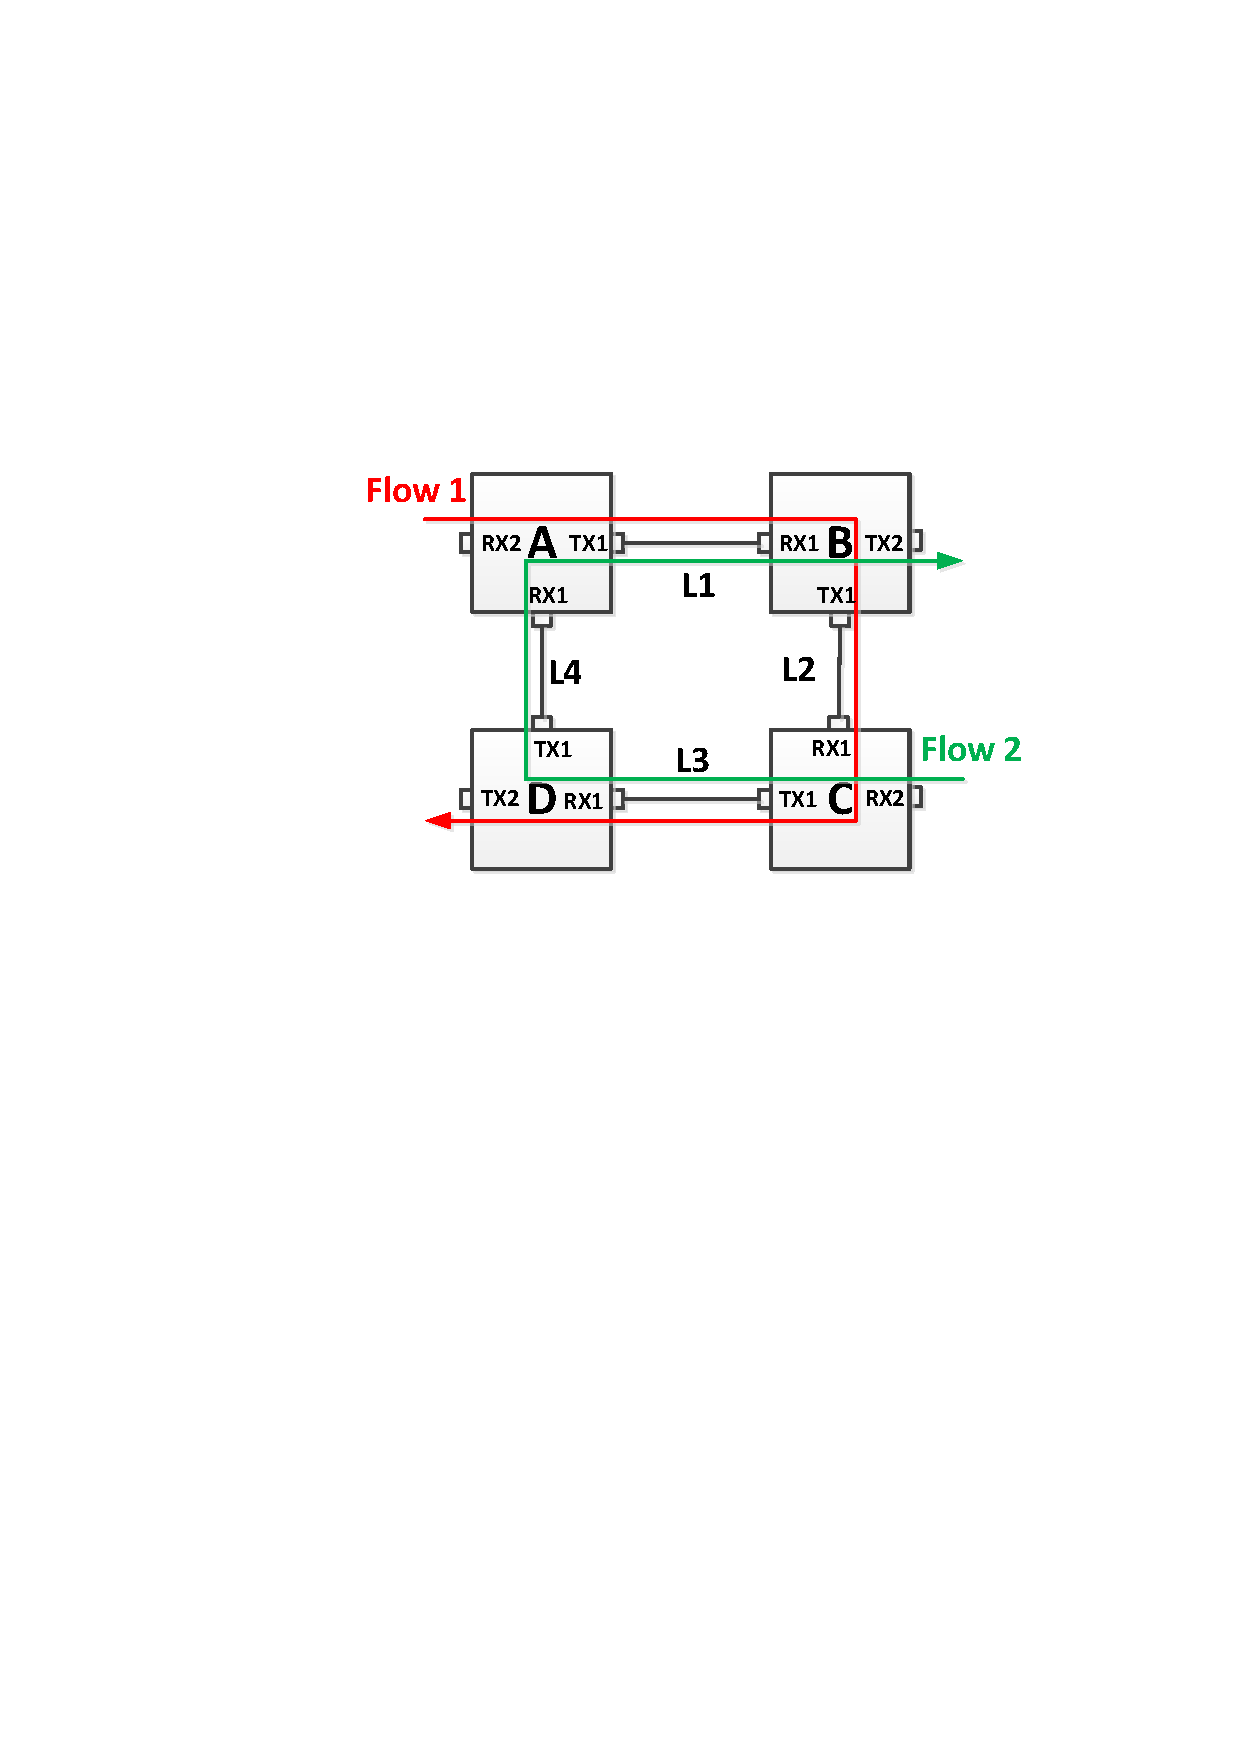
\includegraphics[width=0.3\textwidth] {figs/case1_topo}
%	}
%	\subfloat[short for lof][Buffer dependency graph.]{
%		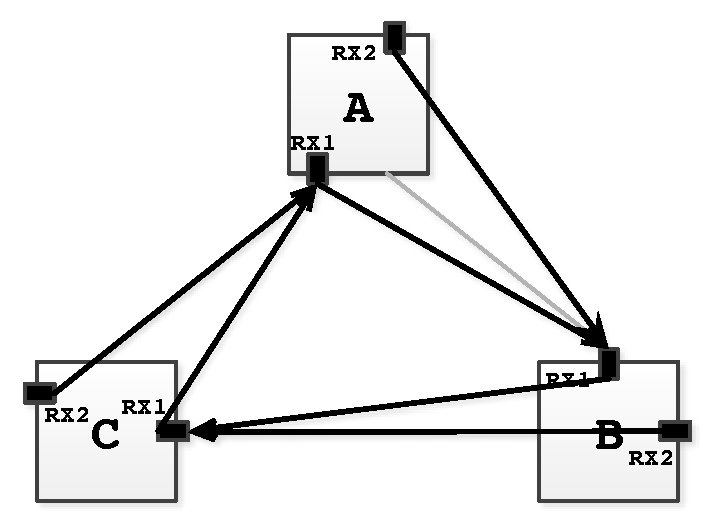
\includegraphics[width=0.2\textwidth] {figs/case1_dependency}
%	}
%	
%	\caption{Flows 1, 2 and 3 forms a cycle in the buffer dependency graph that can create a routing deadlock. In both figures, RX represents an ingress switch queue.}\label{fig:deadlock_case}

%\end{figure}
%
%As shown in Fig.~\ref{fig:deadlock_case}(a), three flows are runing over three switches A, B and C. Flow 1 starts at a host (not shown) attached to A, passes through B, and ends at a host attached to C. Flow 2 and flow 3 are two symmetric flows of flow 1. Buffer dependencies among active ingress queues are drawn in Fig.~\ref{fig:deadlock_case}(b). The path flow 1 takes introduces two dependency links, one from RX2 of A to RX1 of B, the other from RX1 of B to RX1 of C. Similarly, paths taken by flow 2 and flow 3 introduce the other four dependency links in Fig.~\ref{fig:deadlock_case}(b).

%As we can find in Fig.~\ref{fig:deadlock_case}(b), the paths taken by the 3 flows introduce a cyclic buffer dependency among switches A, B and C. When network congestion occurs, it is possible that all the three RX1 queues become full of the packets destined for the next-hop switch and trigger PFC PAUSE simultaneously. Then a PFC deadlock is created as links A-B, B-C and C-A will be permanently paused and no packet in the three RX1 queues can ever get drained.

%\secspace
\section{Potential Deadlock Mitigations}
\label{sec:mitigation}
\secspace

Since cyclic buffer dependency is a loose condition for deadlock, there are
mitigation mechanisms that avoid deadlock even if cyclic buffer dependency is present.
The examples and analysis in Section~\ref{sec:analysis}
inspire us with some of the following potential deadlock mitigations.


\para{TTL-based mitigation for deadlock caused by loops.} In a routing loop, 
the smaller TTL, the less possible deadlock forms (see Equation~\ref{eq:condition}).
Thus, the most straightforward mitigation is to reduce packets' initial TTL values.
For example, in an $N$-hop routing loop, if the initial TTL is not larger than $N$,
no deadlock will form because the deadlock threshold for $r$ is $B$, which can
never be exceeded.

In practice, we may not be able to guarantee that initial TTL values are always smaller than
the size of the loop. However, by proper switch buffer management, we may make {\em class-specific}
TTL much smaller than the actual TTL values. For example, if we assign packets 
that have different TTL values by at least $X$ to different priority classes, the effective TTL becomes $X$
within a priority class. Since PFC PAUSE operates based on priority classes, the deadlock threshold
of injecting rate $r$ is effectively increased.

In worst-case scenarios, the effective TTL may still be larger than the size of loop, meaning
that some $r$ smaller than $B$ leads to deadlock. We may consider rate limiting to keep
$r$ below the threshold $NB/TTL$, as discussed below.

\para{Rate limiting.} Commodity switches support bandwidth shaping for each priority class
or even particular flows. This can mitigate deadlock caused by both routing loops and multi-flow
buffer dependency, as shown in Section~\ref{sec:analysis}. If we are able to predict the rate 
threshold for deadlock, we may bound the individual flow rate by that threshold on switches 
that are involved in cyclic buffer dependency. However, this requires intelligent rate
limiting schemes to avoid over-punishing innocent flows. We leave this to future work.


\para{Limiting PFC pause frames near the source}
PFC is well known for its HoL blocking problem. The damage of HoL and the potential deadlock caused 
by PFC is significant because the pause frames are generated near the destination or in the middle of 
the network, where network congestions usually happen. Hence if we can limit the PFC pause frame 
generation near the source, we can reduce the damage of both deadlock and HoL blocking. 

Here we describe several possible ways of doing so: first, we can assign different PFC thresholds to 
the ports of a switch based on their positions. Ports connecting to the downstream get smaller threshold, 
whereas ports connecting to the upstream get larger threshold. 
Second, we can use switches with larger threshold values at the higher tiers so that they can absorb 
temporal burstiness instead of generating PFC pause frames. Third, again, we may classify 
packets with different TTL into different classes and assign them different PFC thresholds.
Unfortunately, these solutions may lead to other issues including the unfairness between long (across 
different high tier switches) and short ({\em e.g.,} within the same rack) flows. 
This trade-off is less understood and worthy of further study.

% using larger threshold values is tricky, 
%as it does not push PFC back to the source for all cases.)

%In Clos networks, a deadlock that involves high tiers can cause the most serious damage.
%A natural mitigation is to limit the impact of PFC locally near servers. This reduces
%the risk of deadlock as well as the impact once deadlock occurs.
%The idea is to assign different PFC thresholds to different tiers and make PFC happen less
%on higher tier. Also, higher tier switches may be allowed to ignore PFC or drop packets from
%lower tier upon extreme cases.
%The price is that this turns the network into partly
%``lossy'' and may cause congestion drops.

%Second, we may classify packets based on the TTL value they carry, and use TTL-based buffer 
%management similar to that in \ref{karol2003prevention}. The smaller the TTL value of a packet, 
%the smaller the chance that the packet will trigger PFC pause frames. Hence the TTL-based buffer 
%management has the ability to limiting the pause frame generation near the source. But its fairness 
%property is less understood and worthy of further study.

\para{Preventing PFC from been generated.}
The recent transport protocols, DCQCN~\cite{dcqcn} and TIMELY~\cite{timely} are designed to reduce 
the possibility of PFC generation. But due to the feedback 
latency introduced by the end-to-end delay, and the fact that both algorithms react only after the 
congestions have been generated (through either queue length or latency increase), they cannot prevent PFC 
from been generated. 

One possible way to further preventing PFC from been generated is to integrate DCQCN together with 
phantom queuing, like~\cite{Alizadeh12}. By reacting to the phantom queues that assume lower link speed, 
congestion signals are generated much earlier. 

\para{Other possible mechanisms.} In future work, a deeper understanding of tighter conditions 
for deadlock may lead to more deadlock mitigation mechanisms. In future work, we are going to 
investigate the tightest possible conditions -- necessary and sufficient condition for deadlock. 
%\section{Implementation}\label{sec:implementation}

\sysname{} can be implemented by basic match-action functionality
available on most modern commodity switches. However, correct implementation
requires a key insight into the way PFC PAUSE frames are handled.

\begin{figure}
%	\hspace{-0.2in}
	\centering
	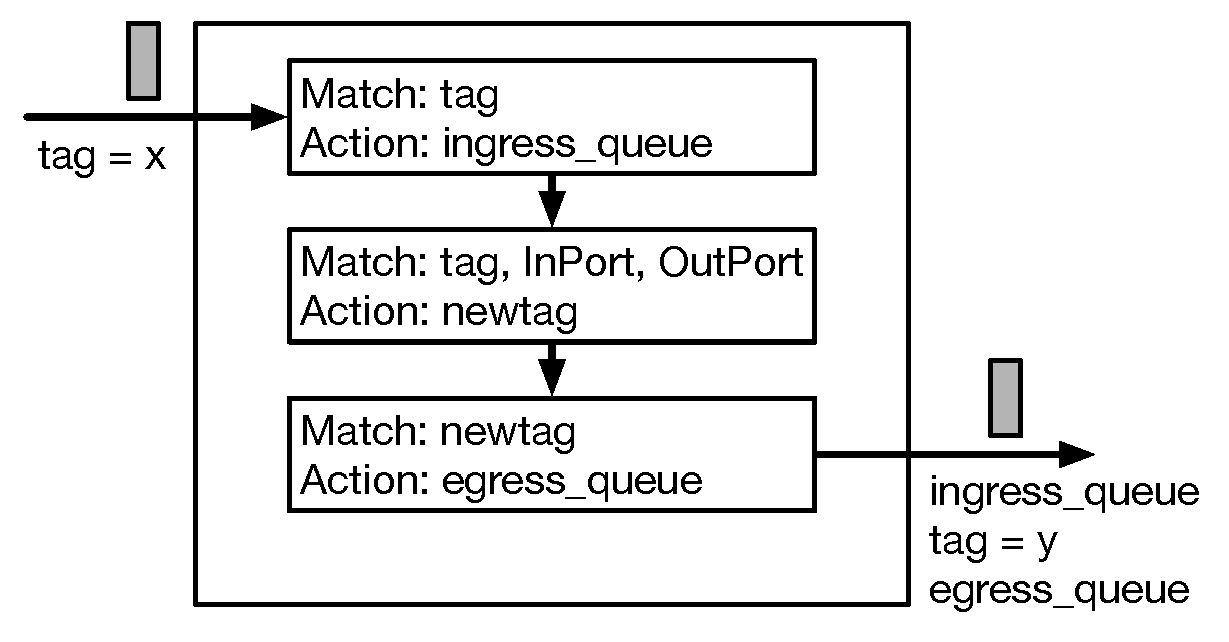
\includegraphics[width=0.42\textwidth] {figs/Tagger}
	%\vspace{-1em}
	\caption{Tagger match-action rules}\label{fig:tagger}
%	\vspace{-2em}
\end{figure}

\para {Match-Action rules:} \sysname{} needs to perform two operations at every
hop, i.e., {\em tag-based priority queueing} and {\em tag
rewriting}.  These two operations are implemented using a 3-step match-action
pipeline (Figure~\ref{fig:tagger}).  First, \sysname{} matches
the value of tags and classifies packets into ingress queues based. Second, 
\sysname{} matches (tag, InPort, OutPort) and rewrites the value of tag. 
The {\em third} step, wherein the packet is placed in an egress queue based on the
{\em new} tag value, is needed to ensure correct PFC operation, as described below.

\begin{figure}[t]
  %\vspace{-3em}
 	\centering
 	\subfloat[short for lof][Ingress priority = egress priority  $\rightarrow$ packet drop.] {
 	%	\vspace{-3em}
 		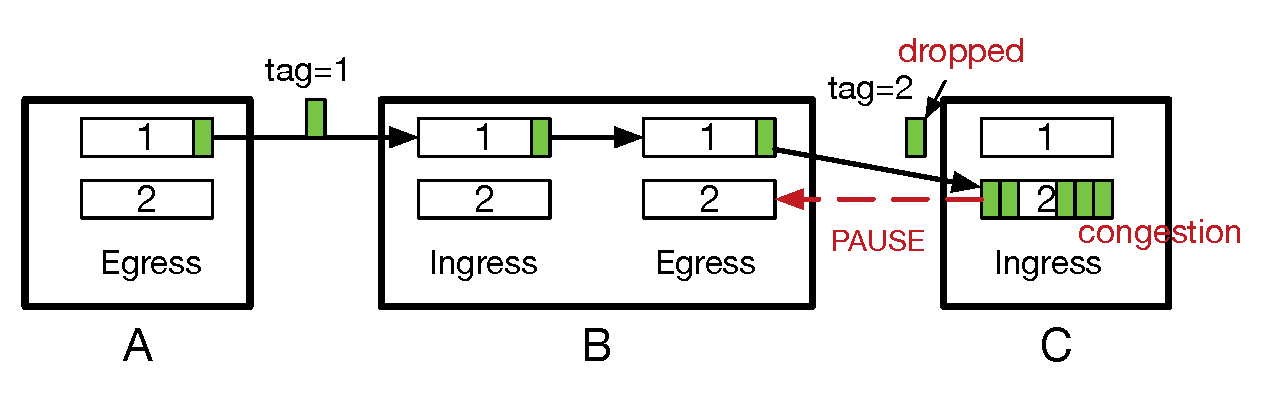
\includegraphics[width=0.42\textwidth] {figs/prioritydecoupling_1}
 	}
%  \vspace{-1.2em}
  
 	\subfloat[short for lof][Ingress priority = 1, egress priority = 2 $\rightarrow$ no drop.]{
 		%\vspace{-3em}
 		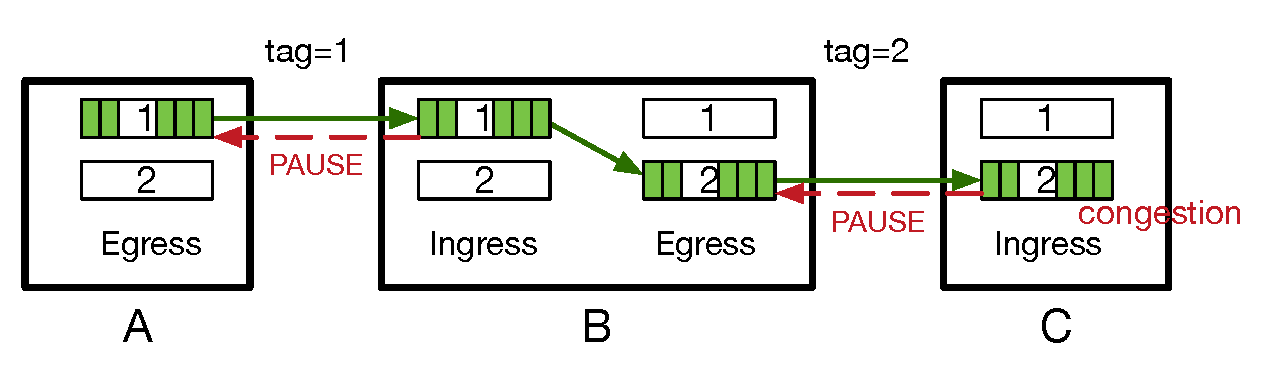
\includegraphics[width=0.42\textwidth] {figs/prioritydecoupling_2}
 	}
	 %\vspace{-1em}
 	\caption{Decoupling ingress priority from egress priority at switch B is necessary for lossless priority transition.}\label{fig:prioritydecoupling}
%	\vspace{-1em}
\end{figure}

\para{Handling priority transition:}
By default, a switch will enqueue a departing packet in the egress queue
of the same priority class as its ingress queue, as shown in Figure~\ref{fig:prioritydecoupling}(a).
In this example, Switch B is configured to 
perform priority transition for packets received from switch A and destined for switch C.
Packets exit egress queue 1 at switch B, but with priority 2. 
When ingress queue 2 of switch C becomes congested, the PFC PAUSE from switch C 
to switch B carries priority 2, and cannot pause the egress queue 1 of switch B.
This default behavior can lead to packet loss.

Therefore, we must map the packet to the egress queue
based on its new priority (Figure~\ref{fig:prioritydecoupling}(b)).  
This avoids packet loss, since the PFC from switch C
correctly pauses the queue on which the packet with the new tag would be
exiting.

\para{Rule compression:}  The match-action rules of \sysname{}
are implemented with TCAM. TCAM entries consist of {\em Pattern},
{\em Mask}, and {\em Result}. They refer to the pattern to be matched, the mask bits 
associated with the pattern and the action that occurs when a lookup hits the pattern, 
respectively.  One TCAM entry can have several Pattern-Mask pairs to match multiple packet header fields
simultaneously, e.g., an entry like (Pattern-1, Mask-1, Pattern-2, Mask-2, Result)
matches two fields simultaneously and fires only if both matches succeed.

\begin{figure}
	 
	\centering
	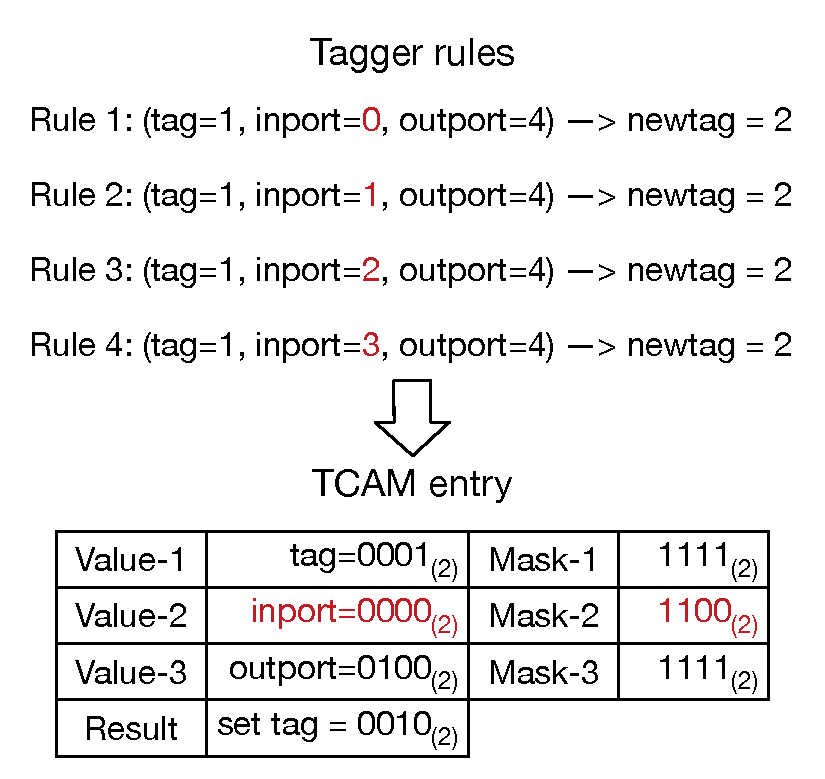
\includegraphics[width=0.37\textwidth] {figs/compression_with_bitmasking}
	\vspace{-1em}
	\caption{Rule compression with bit masking. Port numbers are bitmaps.
	The first bit from right represents port 0. The second bit represents port 1, and so on. }\label{fig:compression}
    \vspace{-1.5em}	
\end{figure}

Rules with the same Result can be compressed into one TCAM entry, if their
Patterns can be aggregated using bit masking. Consider the three
rules in Figure~\ref{fig:compression}. These rules are identical except the InPort
field in Pattern.

On commodity ASICs, port numbers in TCAM are bitmaps, not binary values. To match a single 
port, we can simply set the corresponding bit in the pattern to 1, and set the mask to all 1's. 
However, we may match multiple ports with one rule. We set the pattern to 
all 0's, and set the corresponding bits in the mask to 0. As shown in Figure~\ref{fig:compression},  
to match InPorts 0, 1 and 3, we set Pattern-2 to ``0000''  and Mask-2 to ``0100''. In this case, 
only the packet received from InPorts 0, 1 or 3 will match Pattern-2 after doing bit masking with Mask-2. 
Thus, the three rules are compressed into a single TCAM entry.

Recall from \S\ref{sec:generic} that without any compression, we need
$n(n-1)m(m-1)/2$ rules per switch. The number of rules can be
compressed to $nm(m-1)/2$ by aggregating InPorts.  The
result can be further improved by doing joint aggregation on tag, InPort and
OutPort.

\para{Broadcom implementation:} We implemented \sysname{} on commodity
switches based on Broadcom ASICs.  We use DSCP field in IP header as the tag.
The DSCP-based ingress priority queuing (step 1), ingress ACL and DSCP rewriting (step 2),
and ACL-based egress priority queuing (step 3) are well supported by the
commodity ASICs and do not require any ASIC changes. \shuihai{Everything is implemented using available and documented functionality.}

%Everything is implemented using publicly available and documented functionality.

%DSCP rewriting is supported by all commodity ASICs. DSCP-based priority
%queuing (step 1) is supported natively by all switch ASIC vendors. Step 2 uses
%ingress ACL rules to map (DSCP, InPort, OutPort) to new DSCP.

%Step 3 also uses ACLs, although it relies on certain details that are specific
%to Broadcom's match-action pipeline. We omit these gritty details for brevity.
%While the implementation of this step is Broadcom-specific, we believe that
%ASICs from other vendors can also support this functionality.

%%comment: this claim is not true, as brcm sdk is never public.
%%         
%We stress that none of the three steps require any changes to the switch ASIC,
%and everything is implemented using publicly available and documented
%functionality.

We considered using TTL instead of DSCP to tag packets, but TTL is automatically 
decremented by the forwarding pipeline, which complicates the rule structure.


%\section{Evaluation}\label{sec:eval}

We evaluate \sysname{} using a combination of testbed experiments and numerical
experiments. Our evaluation focuses on three key questions: $(i)$ Can \sysname{}
prevent deadlock? $(ii)$ Is \sysname{} scalable for large data center networks?,
and $(iii)$ Does \sysname{} have a performance penalty?

\begin{figure}
	\centering
	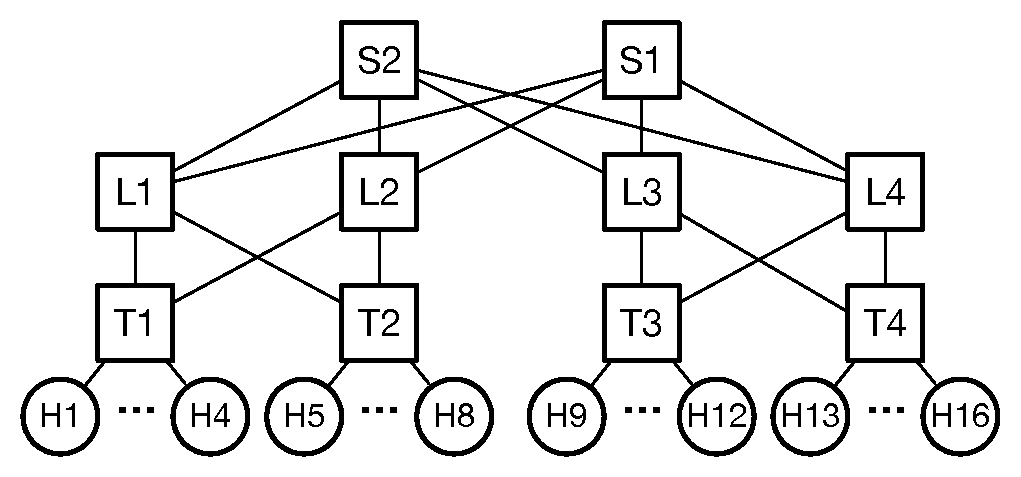
\includegraphics[width=0.45\textwidth] {figs/testbed_topo}
	\caption{Testbed Topology.}\label{fig:testbed_topo}
	\vspace{-0.25in}
\end{figure}

\para{Testbed:} Our testbed consists of a Clos network with 10 switches 16
servers (Figure~\ref{fig:testbed_topo}). Each server is a Dell PowerEdge R730
server with a 40GbE Mellanox ConnectX-3 Pro NIC. Each switch is a Arista
7050 switch with 32 40GbE ports and 16MB packet buffer. The switches
support PFC with at most 8 priority classes.




\subsection{Deadlock prevention}\label{subsec:exp_validation}

\begin{figure}[t]
	%\vspace{-0.1in}
	\centering
	
	\subfloat[short for lof][Without \sysname] {
		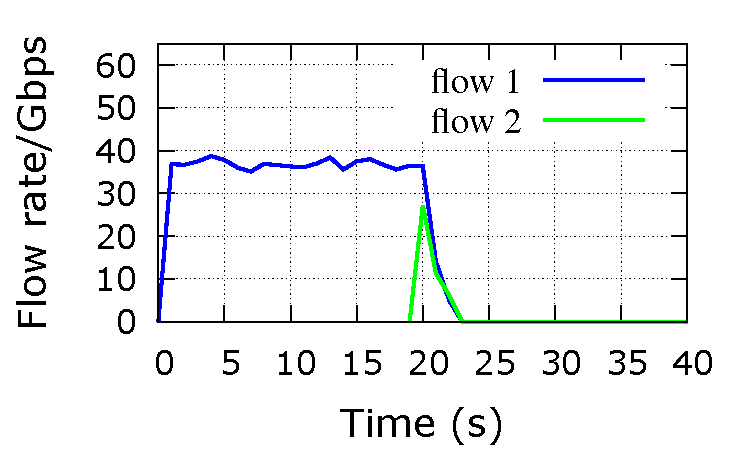
\includegraphics[width=0.25\textwidth] {figs/validation_nonloopcase_flowrate_notagger}
	}
	\subfloat[short for lof][With \sysname]{
		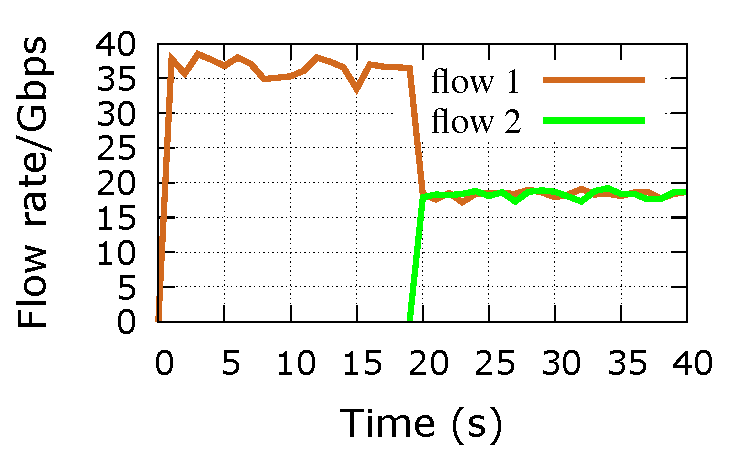
\includegraphics[width=0.25\textwidth] {figs/validation_nonloopcase_flowrate_tagger}
	}
	
	\caption{Clos deadlock due to 1-bounce paths}\label{fig:exp_validation_nonloop}
	\vspace{-0.25in}
\end{figure}

\begin{figure}[t]
	%\vspace{-0.1in}
	\centering
	
	\subfloat[short for lof][Scenario] {
		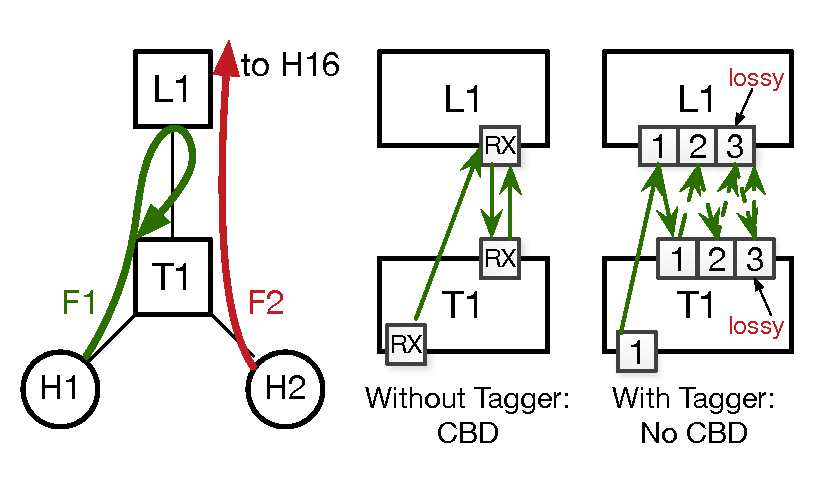
\includegraphics[width=0.4\textwidth] {figs/validation_loopcase_scenario}
	}

\vspace{-0.25in}

	\subfloat[short for lof][Rate of flow 2]{
		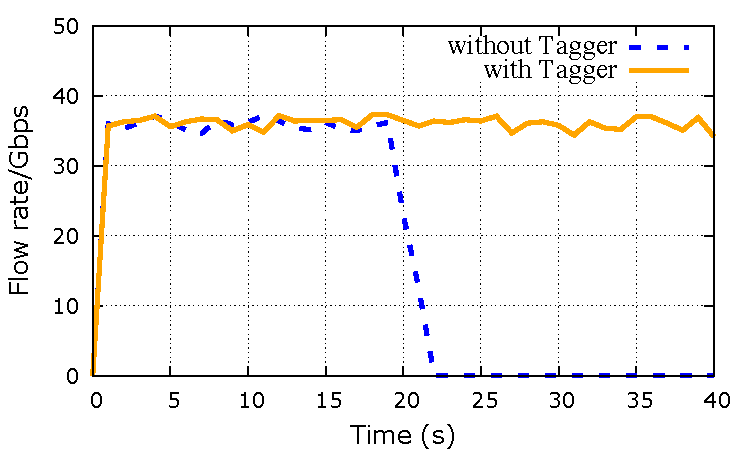
\includegraphics[width=0.4\textwidth] {figs/validation_loopcase_flowrate}
	}
	
	\caption{Deadlock due to routing loop}\label{fig:exp_validation_loop}
	
\end{figure}

\begin{figure}[t]
	%\vspace{-0.1in}
	\centering
	
	\subfloat[short for lof][4-to-1 shuffle with \sysname] {
		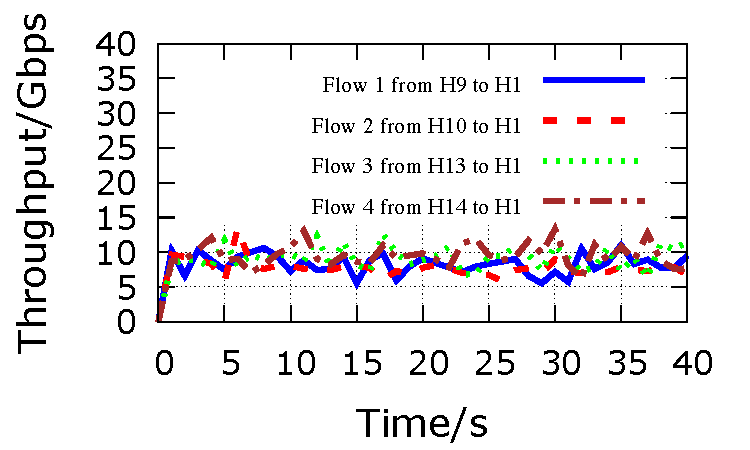
\includegraphics[width=0.25\textwidth] {figs/validation_pp_manytoone_tagger}
	}
	\subfloat[short for lof][4-to-1 shuffle without \sysname]{
		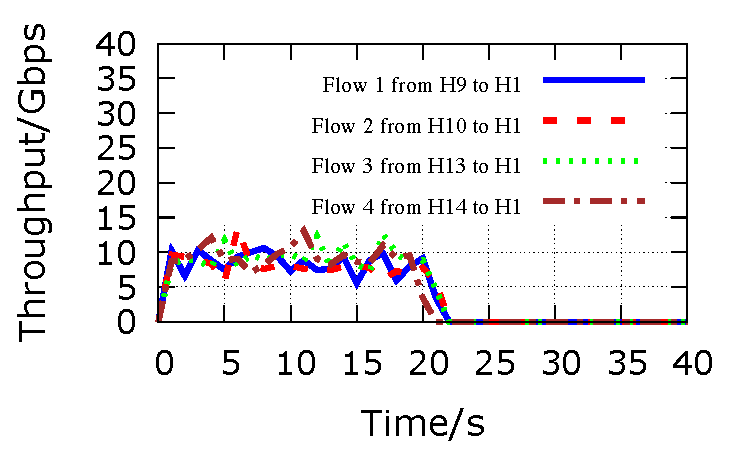
\includegraphics[width=0.25\textwidth] {figs/validation_pp_manytoone_notagger}
	}

	\subfloat[short for lof][1-to-4 shuffle with \sysname] {
	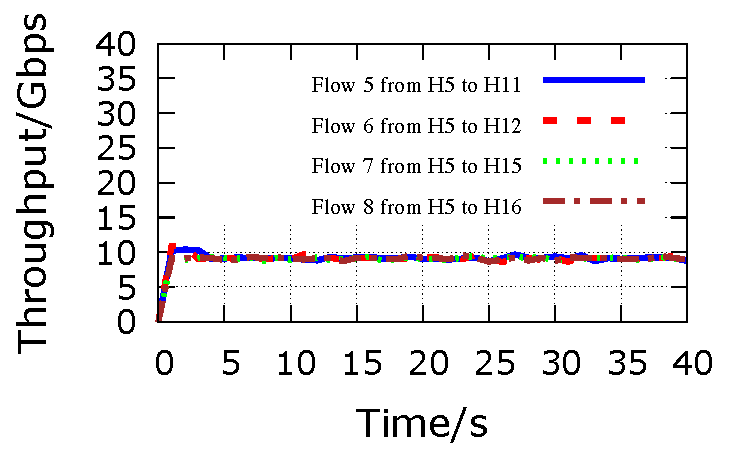
\includegraphics[width=0.25\textwidth] {figs/validation_pp_onetomany_tagger}
}
\subfloat[short for lof][1-to-4 shuffle without \sysname]{
	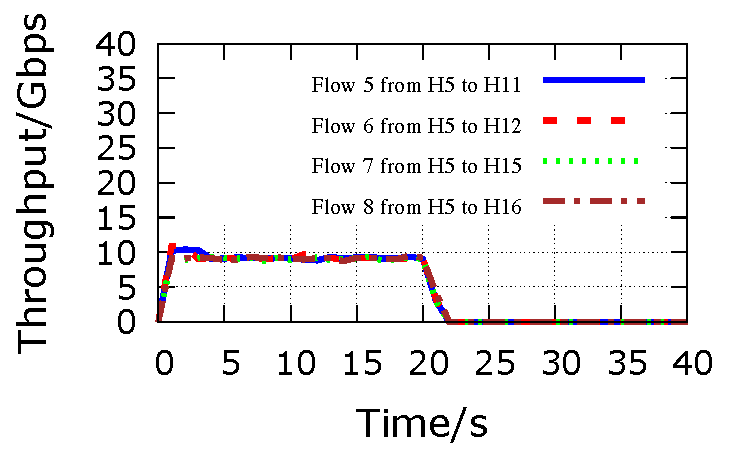
\includegraphics[width=0.25\textwidth] {figs/validation_pp_onetomany_notagger}
}
	
	\caption{PFC PAUSE propagation due to deadlock
	 }\label{fig:exp_validation_propagation}
	
\end{figure}


We have already {\em proved} that \sysname{} prevents deadlock, so the
experiments in this section are primarily illustrative. We have also done
extensive simulations. We omit these for lack of space.

\textbf{Deadlock due to one bounce:} We recreate the scenario shown in
Figure~\ref{fig:clos_1_bounce}, where 1-bounce paths lead to CBD.  In this
experiment, we start the orange flow at time 0, and the green flow at time 20.
Figure~\ref{fig:exp_validation_nonloop} shows the rate of the two flows with and
without \sysname{}.  Without \sysname{}, deadlock occurs and rate of both flows
are reduced to 0. With \sysname{}, and ELR set to include shortest paths and
1-bounce paths, there is no deadlock and flows are not paused.

\textbf{Deadlock due to routing loop:} As shown in
Figure~\ref{fig:exp_validation_loop}(a), we generate 2 flows across different
ToRs, i.e.,  $F_1$ from H1 to H15 and $F_2$ from H2 to H16. At time = 20s, we
install a bad route at L1 to let $F_1$ enter a routing loop between T1 and L1.
The path taken by $F_2$ also traverses link T1-L1.  ELR is set to include the
shortest paths and 1-bounce paths.

In Figure~\ref{fig:exp_validation_loop}(b), we plot the rate of $F_2$ with and
without \sysname{}. As we can see, if \sysname{} is not used, deadlock occurs
and $F_2$ is paused due to propagation of PFC PAUSE. With \sysname{}, there is
no deadlock and $F_2$ is not paused (but rate is affected by the routing loop). Note that
throughput of $F_1$ is zero, as packets are dropped due to TTL expiration.

The key takeaway here is that \sysname{} was able to successfully deal with a
routing loop.

\textbf{PAUSE propagation due to deadlock:} Once deadlock occurs, PFC PAUSE will
propagate and may finally pause all the flow running in the datacenter network.
In this experiment, we run a many-to-one data shuffle from H9, H10, H13 and H14
to H1, and a one-to-many data shuffle from H5 to  H11, H12, H15 and H16
simultaneously.  We then change the routing tables manually so that flow from H9
to H1 and the flow from H5 to H15 take 1-bounce paths. This creates CBD as
discussed earlier.

In Figure~\ref{fig:exp_validation_propagation}, we plot the throughput of all 8
flows with and without \sysname{}. Without \sysname{}, all flows get paused due
to PFC PAUSE propagation and throughput is reduced to zero. With \sysname{},
flows are not affected by link failures.

\subsection{Scalability}
\label{subsec:exp_overhead}

As discussed in \S\ref{sec:challenges}, commodity switches can support only a
limited number of lossless queues.  We have already shown that on a Clos
topology, \sysname{} requires $k+1$ lossless priorities to support paths with
up to $k$ bounces. We now consider other topologies.

\begin{table}[t]
		\footnotesize
	\centering
		\begin{tabular}{|r|r|r|r|r|}
			\hline
				Switches & Ports & Network & Lossless & Max \\
						 &		 & Diameter & Priorities & Rules \\
			\hline
			\hline
			100 & 32 & 6 & 3 &  37 \\
			\hline
			500 & 64 & 6 & 3 & 76 \\
			\hline
			1,000 & 64 & 6 & 3 & 88 \\
			\hline
			2,000 & 64 & 7 & 3 & 98 \\
			\hline
			2,000 (*)  & 64 & 7 & 4 &  135\\
			\hline
			
		\end{tabular} 
		\caption{Rules and priorities required for Jellyfish. Half the ports on
		each switch are connected to servers. ELP is shortest paths for first four entries. ELP for last entry includes additional 20,000 random paths.}
\label{table:jellyfish_shortestpath} \end{table}

Jellyfish topology is an r-regular random graph, characterized by the number of
switches, the number of ports a switch has (n) and the number of ports used to
connect with other switches (r).  In our experiment, we let r = n/2. Remaining
ports are connected to servers. We construct ELP by building destination-rooted
shortest-path spanning trees at all the servers.
Table~\ref{table:jellyfish_shortestpath} shows the results.  

\sysname{} requires only four classes for a network with 2000 switches, even
when 20,000 random routes are used in addition to the shortest paths, and at
most\footnote{Different switches require different number of rules due to the
random nature of the topology.} 135 match-action rules per switch.  Modern
commodity switches can support 1-4K rules, so this is not an issue. 

We also considered smaller (100 switches, 32 ports) Jellyfish topologies with
upto 16-shortest path routing. We need just 2 lossless priorities, and no more
than 47 rules per switch.

BCube~\cite{bcube} is server-centric topology, constructed from servers with $n$
ports, $n^k$ switches with $n$ ports. BCube$(8,3)$ with ELP of $3$ shortest
paths requires 4 lossless priorities, and 41 rules per switch.
F10~\cite{f10} is a fault-tolerant FatTree-like topology.  With three-level
network of 64 port switches, and ELP of all shortest and 1-bounce paths, we need
just 2 lossless priorities and 164 rules per switch.

Generating tagging rules is a one-time activity. Still, runtime of
Algorithm~\ref{alg:greedy} is of possible interest.
Figure.~\ref{fig:algo_runtime} shows the runtime for Jellyfish topologies of
different sizes. Even with 2000 switches, we complete rule generation in about
1.5 hours on a commodity desktop machine.

Thus, we conclude that in terms of number of lossless classes and ACLs,
\sysname{} scales well for modern data center architectures. 

\begin{figure}
	\centering
	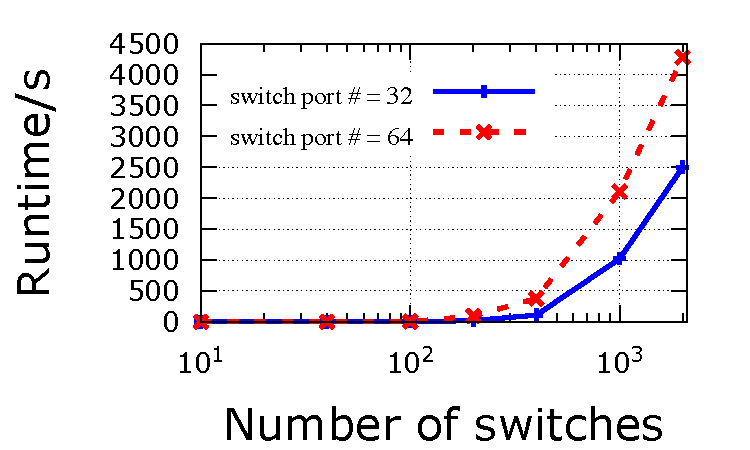
\includegraphics[width=0.45\textwidth] {figs/algo_runtime}
	\caption{Runtime of Algorithm~\ref{alg:greedy} for Jellyfish network of different sizes.}
	\label{fig:algo_runtime}
	\vspace{-0.25in}
\end{figure}

\subsection{Impact on throughout and latency}\label{subsec:exp_performanceoverhead}

\begin{figure}[t]
	\centering
	
	\subfloat[short for lof][Throughput] {
		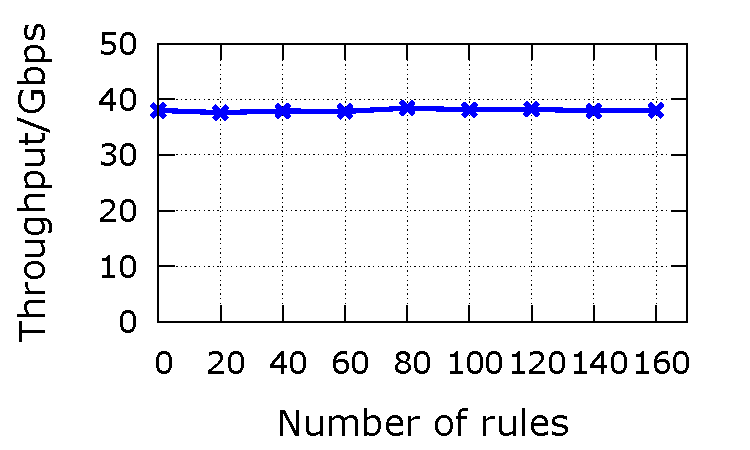
\includegraphics[width=0.25\textwidth] {figs/overhead_avgthrpt}
	}
	\subfloat[short for lof][Latency]{
		\includegraphics[width=0.25\textwidth] {figs/RDMAlatency_overhead}
	}
	
		\caption{\sysname{} has no impact on throughput and latency}
		\label{fig:perf_penalty}
	\vspace{-0.25in}
\end{figure}

At run time, the only impact of \sysname{} is that the packet has to traverse
the ACL rules. These are installed in TCAM, and hence have no discernible impact
on throughput and latency, as illustrated in Figure~\ref{fig:perf_penalty}.

\textbf{Throughput}: We generate one flow from H1 to H2, and observe its average
throughput over 100 seconds under varying number of \sysname{} rules installed
on T1. Figure~\ref{fig:perf_penalty}(a) shows that the average throughput is not
affected.

\textbf{Latency}: We install different number of \sysname{} rules in T1 and
collect 5000 RTT samples between H1 and H2.  Table~\ref{fig:perf_penalty}(b)
shows that latency is not affected.



%\subsection{Simple demonstration of \sysname{}}\label{subsec:exp_demon}  
%	
%	\begin{figure}[t]
%		%\vspace{-0.1in}
%		\centering
%		
%		\subfloat[short for lof][Experiment scenario.]{
%			\includegraphics[width=0.25\textwidth] {figs/demon_scenario}
%		}
%		\subfloat[short for lof][Rate of flow 1 and flow 2.]{
%			\includegraphics[width=0.25\textwidth] {figs/demon_flowrate}
%		}
%		
%		\caption{The match-action rules in action}\label{fig:tagger_demon}
%	\end{figure}
%	
%	
%A simple experiment shown in
%Figure~\ref{fig:tagger_demon} demonstrates the behavior of the match-action
%rules.  We generate two flows, flow 1 and flow 2, to send packets to C from
%different servers connected to ports A and B. Both servers set the DSCP value in
%outgoing packets to 1. The match-action rules are set to rewrite the tag value
%of packets arriving on port A to 2, and forward them to port C. Tag of packets
%arriving on port B is not changed.
%
%At time = 17s, C sends a stream of forged PFC PAUSE frames on priority 2 to
%switch S. The rate of both flows is plotted in Figure~\ref{fig:tagger_demon}(b)
%(link capacity = 40Gbps). As expected, after priority 2 is paused, rate of
%flow 1 is reduced to 0 while flow 2 gets all the available bandwidth.
%Counters on switch S further confirm that no packets were dropped, and server
%connected to port A was paused as expected.

%%\vspace{-0.1in}
\section{\sys Applications}\label{sec:application}
%\vspace{-0.1in}
To showcase \sys's utility, we use it for explicit path support in four applications. The key is that, built on \sys, applications can freely choose which path to use without worrying about how to set up the path and the time cost or overhead of setting up the path. In this regard, \sys emerges as an interface for applications to use explicit paths conveniently, but does not make any choice on behalf of them.

%We incorporate \sys into 5 representative applications for routing and demonstrate its utility. For bandwidth-guarantee, we show that \sys's explicit path control makes end-to-end bandwidth provisioning easier to implement. For partition-aggregation application, we show that \sys can express 1-to-$n$ or $n$-to-1 patterns and can be leveraged to give search query high priority for service differentiation. For map-reduce, we show that \sys can express $m$-to-$n$ pattern and the path IDs can used to identify disjoint parallel paths that speedup the many-to-many data shuffle and avoid collision of ECMP.

%\begin{figure}[t]
%\centering
%\subfloat[nooneline, footnotesize][Remaining bandwidth on $P_1$, $P_2$, $P_3$ is 300, 100, 100 Mbps.]
%{\includegraphics[width=0.28\textwidth] {figs/iops-topo.eps}}
%%\vspace{-0.1in}
%\subfloat[nooneline, footnotesize][Average IOPS.] {
%{\scalebox{0.8} {
%\begin{tabular}[b]{|l | c|}
%    \hline
%    & \tabincell{c}{\textbf{Average IOPS}} \\
%    \hline
%    \hline
%    \sys & 15274 \\
%    \hline
%    ECMP & 4547 \\
%    \hline
%\end{tabular}}}}
%
%\subfloat[nooneline, footnotesize][Throughput and completion time of RoX and ECMP.] {
%\includegraphics[width=0.45\textwidth]{figs/iops-throughput.eps}}
%%\vspace{-0.17in}
%\caption{\sys utility case $\#1$: we leverage \sys to make provisioned I/O bandwidth easier to implement.}
%\end{figure}

%\vspace{-0.1in}
\subsection{\sys for provisioned IOPS}\label{subsec:iops}
%\vspace{-0.1in}
%In cloud services, there is an increasing need for bandwidth provisioning. For example, Amazon RDS enforces provisioned I/O bandwidth for instances to ensure that disk resources are always available whenever you need them~\cite{privisionIO}. In this experiment, we show \sys's explicit path control makes end-to-end bandwidth provisioning easy to implement. For the experiment setting, we pick a pod and use background UDP flows to stature the ToR-Agg links and leave the remaining bandwidth on three paths between X-Y as 100Mpbs, 300Mbps, 100Mbps respectively. Suppose now there comes a demand to provision the bandwidth between X-Y at 300Mbps. We then leverage ECMP and \sys to implement it.

\begin{figure}[t]
\centering
%\vspace{-0.1in}
\includegraphics[width=0.5\textwidth,center]{figs/f8.eps}\hspace{-0.2in}
%\vspace{-0.1in}
\caption[Optional caption for list of figures]{\sys utility case $\#1$: we leverage \sys to make necessary bandwidth easier to implement for provisioned IOPS.}
\label{fig:iops}
\vspace{-0.2in}
\end{figure}

In cloud services, there is an increasing need for provisioned IOPS. For example, Amazon EBS enforces provisioned IOPS for instances to ensure that disk resources can be accessed with high and consistent I/O performance whenever you need them~\cite{privisionIO-EBS}. To enforce such provisioned IOPS, it should first provide necessary bandwidth for the instances~\cite{io-characteristics}. In this experiment, we show \sys can be easily leveraged to use the explicit path with necessary bandwidth.

As shown in Fig.~\ref{fig:iops}(a), we use background UDP flows to stature the ToR-Agg links and leave the remaining bandwidth on 3 paths ($P_1, P_2$ and $P_3$) between X-Y as 300Mpbs, 100Mbps, and 100Mbps respectively. Suppose there is a request for provisioned IOPS that requires 500Mbps necessary bandwidth (The provisioned IOPS is about 15000 and the chunk size is 4KB.). We now leverage \sys and ECMP to write 15GB data ($\approx$4 million chunks) through 30 flows from X to Y, and measure the achieved IOPS respectively. The storage we used for the experiment is Kingston V+200 120G SSD, and the I/O operations on the storage are sequential read and sequential write.

\begin{figure}[t]
\centering
\vspace{-0.15in}
\subfloat[short for lof][Path $P_1$: T1~$\rightarrow$A1~$\rightarrow$T3; $P_2$: T1~$\rightarrow$A2~$\rightarrow$T3; $P_3$: T1~$\rightarrow$A3~$\rightarrow$T3] {
    \includegraphics[width=0.40\textwidth] {figs/updt-topo.eps}
    \label{fig:network-update_a}
}
\vspace{-0.15in}

\subfloat[short for lof][Time $t_1$: move $f_3$ from $P_2$ to $P_3$;~ $t_2$: move $f_1$ from $P_1$ to $P_2$;~$t_3$: move $f_1$ from $P_2$ to $P_1$;~ $t_4$: move $f_3$ from $P_3$ to $P_2$.]{
    \includegraphics[width=0.40\textwidth] {figs/updt-mat-new.eps}
    \label{fig:network-update_b}
}
\vspace{-0.1in}
\caption[Optional caption for list of figures]{\sys utility case \#2: we leverage XPath to assist zUpdate~\cite{zupdate} to accomplish DCN update with zero loss.}
\label{fig:network-update}
\vspace{-0.2in}
\end{figure}

From Fig.~\ref{fig:iops}(c), it can be seen that using ECMP we cannot provide the necessary bandwidth between X-Y for the provisioned IOPS although the physical capacity is there. Thus, the actual achieved IOPS is only 4547, and the write under ECMP takes much longer time than that under \sys as shown in Fig.~\ref{fig:iops}(c). This is because ECMP performs random hashing and cannot specify the explicit path to use, hence it cannot accurately make use of the remaining bandwidth on each of the multiple paths for end-to-end bandwidth provisioning. In contrast, \sys can be easily leveraged to provide the required bandwidth due to its explicit path control. With \sys, we explicitly control how to use the three paths and accurately provide 500Mbps necessary bandwidth, achieving 15274 IOPS.


%\vspace{-0.05in}
\subsection{\sys for network updating}\label{subsec:update}
\vspace{-0.05in}
In production data centers, DCN update occurs frequently~\cite{zupdate}. It can be triggered by the operators, applications and various networking failures. zUpdate~\cite{zupdate} is an application that aims to perform congestion-free network-wide traffic migration during DCN updates with zero loss and zero human effort. In order to achieve its goal, zUpdate requires explicit routing path control over the underlying DCNs. In this experiment, we show how \sys assists zUpdate to accomplish DCN update and use a switch firmware upgrade example to show how traffic migration is conducted with \sys.

In Fig.~\ref{fig:network-update}(a), initially we assume 4 flows ($f_1, f_2, f_3$ and $f_4$) on three paths ($P_1, P_2$ and $P_3$). Then we move $f_1$ away from switch $A_1$ to do a firmware upgrade for switch $A_1$. However, neither $P_2$ nor $P_3$ has enough spare bandwidth to accommodate $f_1$ at this point of time. Therefore we need to move $f_3$ from $P_2$ to $P_3$ in advance. Finally, after the completion of firmware upgrade, we move all the flows back to original paths. We leverage \sys to implement the whole movement.

\begin{figure}[t]
\centering
%\vspace{-0.2in}
\includegraphics[width=0.45\textwidth]{figs/be.eps}
%\vspace{-0.15in}
\caption{\sys utility case $\#3$: we leverage \sys to accurately enforce VDC with bandwidth guarantees.}
\label{fig:bandwidth_enforcement}
\vspace{-0.2in}
\end{figure}

In Fig.~\ref{fig:network-update}(b), we depict the link utilization dynamics. At time $t_1$, when $f_3$ is moved from $P_2$ to $P_3$, the link utilization of $P_2$ drops from 0.6 to 0.4 and the link utilization of $P_3$ increases from 0.7 to 0.9. At time $t_2$, when $f_1$ is moved from $P_1$ to $P_2$, the link utilization of $P_1$ drops from 0.5 to 0 and the link utilization of $P_2$ increases from 0.4 to 0.9. The figure also shows the changes of the link utilization at time $t_3$ and $t_4$ when moving $f_3$ back to $P_2$ and $f_1$ back to $P_1$. It is easy to see that with the help of \sys, $P_1, P_2$ and $P_3$ see no congestion and DCN update proceeds smoothly without loss.

%Compared to OpenFlow, since \sys is capable to pre-install large number of paths into IP tables, zUpdate doesn't need to change the flow and group tables on switches in every step of the traffic migration. For most of the cases, \sys only needs to notify the senders to transfer a part of flows to some other paths.

%\vspace{-0.1in}
\subsection{Virtual network enforcement with \sys}\label{subsec:vne}
%\vspace{-0.05in}
%
%\begin{figure*}[ht]
%\centering
%\subfloat[short for lof][The Fattree(6) testbed with 54 servers we implemented. Each ToR switch connects 3 servers (not drawn).] {
%    \includegraphics[width=0.32\textwidth] {figs/testbed-topo}
%    \label{fig:fattree}
%}
%\vspace{-0.17in}\hfill
%\subfloat[short for lof][\sys utility case $\#4$: we leverage \sys to express partition-aggregation traffic pattern ($1$-to-$n$, $n$-to-$1$) and enforce service differentiation.] {
%    \includegraphics[width=0.33\textwidth] {figs/pa.eps}
%    \label{fig:partition_aggregation_query}
%}\hfill
%\subfloat[short for lof][\sys utility case $\#5$: we leverage \sys to select non-conflict paths to speed up many-to-many data shuffle.]{
%    \includegraphics[width=0.3\textwidth] {figs/shuffle}
%    \label{fig:shuffle}
%}
%\caption[Optional caption for list of figures]{}
%\label{fig:network-update}
%\vspace{-0.2in}
%\end{figure*}


In cloud computing, virtual data center (VDC) abstraction with bandwidth guarantees is an appealing model due to its performance predictability in shared environments~\cite{secondnet,oktopus,proteus2012}. In this experiment, we show \sys can be applied to enforce virtual networks with bandwidth guarantees. We assume a simple SecondNet-based VDC model with 4 virtual links, and the bandwidth requirements on them are 50Mbps, 200Mbps, 250Mbps and 400Mbps respectively as shown in Fig.~\ref{fig:bandwidth_enforcement}(a). We then leverage \sys's explicit path control to embed this VDC into the physical topology.

In Fig.~\ref{fig:bandwidth_enforcement}(b), we show that \sys can easily be employed to use the explicit paths in the physical topology with enough bandwidth to embed the virtual links. In Fig.~\ref{fig:bandwidth_enforcement}(c), we measure the actual bandwidth for each virtual link and show that the desired bandwidth is accurately enforced. However, we found that ECMP cannot be used to accurately enable this because ECMP cannot control paths explicitly.

%\vspace{-0.2in}
%\subsection{\sys support for partition-aggregation query}\label{subsec:partition}
%\vspace{-0.1in}
%In web applications, the partition-aggregation paradigm is a foundation for many online services such as search query. They usually generate one-to-many and many-to-one communication patterns and has very demanding latency requirements. Using \sys, we can explicitly express such 1-to-$n$ and $n$-to-1 patterns using ($n$+1) path IDs, one ID for $n$-to-1 and $n$ IDs for 1-to-$n$. These IDs form a group that can be leveraged for optimizations such as service differentiation.
%
%In this experiment, we selected 9 servers in a pod to emulate a 1-to-8 (8-to-1) query-and-response, and we used 9 IDs to express such group communication patterns. We saturate the network with background traffic, and then leverage such 9 IDs to set priority to such query-and-response traffic.
%
%\begin{figure}[t]
%\vspace{-0.1in}
%\centering
%\includegraphics[width=0.45\textwidth]{figs/pa.eps}
%\vspace{-0.1in}
%\caption{\sys utility case $\#4$: we leverage \sys to express partition-aggregation traffic pattern ($1$-to-$n$, $n$-to-$1$) and enforce service differentiation.}
%\label{fig:partition_aggregation_query}
%\vspace{-0.25in}
%\end{figure}
%
%
%
%In Fig.~\ref{fig:partition_aggregation_query}, we found that when the group of path IDs are referenced for priority, the query flows see persistently low RTTs of less than 200$\mu$s irrespective of the background traffic. However, if we do not set up a priority for these IDs, the RTT increases to the millisecond level as the background load increases. This experiment showcases \sys's utility in service differentiation for partition-aggregation queries.

%\vspace{-0.1in}
\subsection{Map-reduce data shuffle with \sys}\label{mapreduce}
%\vspace{-0.1in}
In Map-reduce applications, many-to-many data shuffle between the map and reduce stages can be time-consuming. For example, Hadoop traces from Facebook show that, on average, transferring data between successive stages accounts for $33\%$ of the running times of jobs~\cite{orchestra}. Using \sys, we can explicitly express non-conflict parallel paths to speed up such many-to-many data shuffle. Usually, for a $m$-to-$n$ data shuffle, we can use ($m$+$n$) path IDs to express the communication patterns. The shuffle patterns can be predicted using existing techniques~\cite{hadoopwatch}.

\begin{figure}[t]
%\vspace{-0.1in}
\centering
\includegraphics[width=0.5\textwidth]{figs/shuffle}
\vspace{-0.2in}
\caption{\sys utility case $\#4$: we leverage \sys to select non-conflict paths to speed up many-to-many data shuffle.}
\label{fig:shuffle}
\vspace{-0.2in}
\end{figure}

In this experiment, we selected 18 servers in two pods of the Fattree to emulate a 9-to-9 data shuffle by letting 9 servers in one pod send data to 9 servers in the other pod. We varied the data volume from 40G to over 400G. We compared \sys with ECMP.

In Fig.~\ref{fig:shuffle}, it can be seen that by using \sys for data shuffle, we can perform considerably better than randomized ECMP hash-based routing. More specifically, it reduces the shuffle time by over 3$\times$ for most of the experiments. The reason is that \sys's explicit path IDs can be easily leveraged to arrange non-interfering paths for shuffling, thus the network bisection bandwidth is fully utilized for speedup.


%We further note that \sys can simply use 3 path IDs to express such many-to-many communication patterns, which makes the non-conflict parallel path arrangement fairly easy to implement.



%%\vspace{-0.1in}
\section{Related Work}\label{sec:related}

\para{Deadlock-free routing.} Many Deadlock-free routing designs have been
proposed. See
\cite{dally,duato93,dally93,sancho2004,flich2012survey,lash,wu2003fault,glass,duato2001,domke2011,puente1999,dfedst16}
for representative schemes. Generally, these designs prevent deadlock by
imposing restrictions on the routing paths, and can be classified into two
categories.

The first category is {\em deterministic routing based approach}, in which the
routing path is not affected by the traffic status, and there is no CBD.  These
routing algorithms are not compatible with existing routing protocols including
OSFP and BGP. Worse, they cannot be implemented in current commodity switching
ASICs.

TCP-Bolt~\cite{tcpbolt} and DF-EDST~\cite{dfedst16} are two recently
proposed deadlock-free routing designs. They both build edge-disjoint
spanning trees (EDSTs), with DF-EDST~\cite{dfedst16} further builds a
deadlock-free tree transition acyclic graph such that the transition
among some EDSTs can be allowed. However, existing L3 routing protocols
do not guarantee that packets will follow the pre-assign EDSTs, especially
upon link failures. Current switching ASIC cannot detect and handle all 
the potential EDST transition properly.

%support EDST.
%Furthermore, these designs need many EDSTs and
%every EDST needs to occupy a lossless queue. 
%Current switching ASIC,
%however, can only support 2-3 lossless queues.

The second category is {\em adaptive routing based approach.} The key idea is to
pre-install  ``escape'' paths at every switch to cover all possible
destinations. The switches can reroute packets to the ``escape'' paths in the
presence of congestion so that deadlock can be avoided.  As far as we know, no
commodity switching ASIC supports dynamic reroute based on traffic / queue
status.

\para{Intel Omni-Path.} Intel Omni-Path architecture \cite{omnipath} uses the
concept of Service Channels (SC) for routing deadlock avoidance.  Unlike
\sysname{}, Ommi-path uses a centralized fabric manager to manage the
network~\cite{omnipath}, including setting up SCs. This is not feasible at
data center scale.

%% Technical details of Omni-Path are not currently available, Tagger differs
%% from Omni-Path in two significant ways. First, Omni-path needs a fabric
%% manager to dynamically setup SC whereas the tag match-action rules are
%% pre-computed and statically configured. Second, Tagger enforces that
%% the tag of a packet increases monotonically whereas Omni-Path does not
%% enforce order for SC.

\para{Buffer management for deadlock prevention.} It has been shown that by
increasing the packet priority hop-by-hop, and putting packets of different
priority into different buffers, deadlock can be avoided
\cite{firstpaper,survey,datanetworks,karol2003prevention}. These designs,
however, need a large number lossless queues (which is the diameter of the
network). In \cite{dag}, the author tried to reduce the number of lossless
queues to only two. The design does not guarantee losslessness. Furthermore,
some switches need much larger buffer space than the others. 

\para{Deadlock recovery.} Deadlock recovery schemes
\cite{isca95,shpiner2016unlocking,venkatramani1996,martinez1997,Lopez1998}
detect deadlocks once they occur, and then try to break them by rerouting
packets.  These approaches have two issues: (1) They cannot guarantee that
deadlock will not happen again (if they can, there will be no need for deadlock
recovery). (2) They cannot be deployed using existing switch hardware.

%% need to add new deadlock detection algorithms and deadlock
%% breaking protocols into the switches.

%\para{Circuit switching-based approaches.} Those solutions from HPC and InfiniBand
%work by preemption. This does not work in Ethernet and in practice.

\para{Deadlock-free routing reconfiguration}:
Several deadlock-free routing reconfiguration schemes
\cite{automatic,lysne2005,doublescheme,gara2005} have been proposed for
ensuring deadlock-free during routing reconfiguration. \sysname{} can
be used to help any routing protocol to be deadlock-free, as
\sysname{} is decoupled from the routing protocols.

%The basic idea is to divide the reconfiguration process into multiple
%stages, and guarantee deadlock-free routing within each stage. We
%believe
%\sysname{} can be easily modified to guarantee deadlock-free of each
%reconfiguration stage.

\para{Summary.} \sysname{} is different from prior work because it works with
any routing protocol, and with existing hardware. We further have shown that
\sysname{} needs only small number of lossless queues.

%We believe that deciding the priority of packets along the path is
%better than changing routing configurations.

%Deadlock-free routing \cite{dally,duato93,dally93,sancho2004,flich2012survey,lash,wu2003fault,glass,duato2001,domke2011,puente1999} can be achieved by splitting the physical links into virtual channels and virtual channels are arranged in a way so as to avoid circular buffer dependency. In all those designs, the routing is decided by the virtual channels. Hence they cannot work with existing routing protocols for the data center networks which was designed for the lossy networks.
%can be achieved by splitting the physical links into virtual channels and virtual channels are arranged in a way so as to avoid circular buffer dependency. In all those designs, the routing is decided by the virtual channels. Hence they cannot work with existing routing protocols for the data center networks which was designed for the lossy networks.

%%TCP-Bolt~\cite{tcpbolt} uses multiple edge-disjoint spanning trees (EDSTs) and puts every EDST into a separate VLAN and lossless queue to achieve deadlock-free. In addition to the above drawbacks, to achieve good performance, TCP-Bolt may need a large number of lossless queues (which cannot be provided in current commodity switches). Furthermore, TCP-Bolt needs to run layer-2 VLAN, whereas all large-scale data center networks run layer-3.
%
%%DF-EDST~\cite{dfedst16} introduces a set of edge-disjoint spanning trees and a tree transition graph to provide deadlock free routing for arbitrary data center network topologies. DF-EDST, however, cannot work with existing routing protocols as it needs to follow the EDSTs. Furthermore, The EDST selection and transition cannot be readily implemented in current Ethernet switches.

%\secspacelarge
\section{Conclusion}
\secspace

In this paper, we studied the problem of deadlock in datacenter networks.  We
showed that CBD is a {\em necessary} by not {\em
sufficient} condition for deadlock formation. We are unable to fully characterize
the sufficient conditions, but using insights gained from a few examples, we
discussed potential deadlock mitigation mechanisms including TTL-based schemes,
rate limiting and reducing PFC propagation.



%\vspace{0.1in}
%\section*{Acknowledgements}


%\begin{normalsize}
%\begin{small}
	\bibliographystyle{plain}
	\bibliography{reference}
%\end{small}
%\end{normalsize}
%\begin{appendices}
\section{PFC headroom calculation}\label{APPHEADROOM}

The PFC headroom needed per port per lossless queue can be calculated by
		considering the time interval needed for a receiver to pause its
		upstream sender. The time interval is composed of the following 6
		periods for the lossless class $p$:

	
\noindent\textbf{The time to send a PAUSE frame $t_1$}.  Once a pause frame is
		generated, it may be blocked by a packet that has just started
		transmision. Since Ethernet is non-preemptive, in the worst-cast,
		$t_1 = \frac{ L_{mtu} + L_{pfc}}{B}$, where $L_{mtu}$ is the MTU size,
		and $L_{pfc}$ is the size of a PFC pause frame, and $B$ is the link
		rate.


\noindent\textbf{The PAUSE frame propagation time $t_2$}. This depends on 
		the cable length between the sender and receiver.

\noindent\textbf{The PAUSE frame receiving time at the sender $t3$}.
		$t_3=\frac{L_{pfc}}{B}$.

\noindent\textbf{The PFC response time $t_4$}. This is the amount of time needed
		for the sender to process the pause frame.

\noindent\textbf{The time for the sender to stop transmitting $t_5$}. Again,
		because Ethernet is non-preemptive, sender must to finish 
		transmitting the packet that may have already started. Hence, in the
		worst case, $t_5 =
		\frac{L^{p}_{mtu}}{B}$.

\noindent\textbf{The time for the pipe to be drained $t_6$}. We know $t_6 =
		t_2$.


At a first glance, the headroom size should be $B\times\sum t_i$. But there are
some additional details. The switching ASICs typically divide a packet
into small cells of equal size for internal packet storage and
processing. The cell size ($C$) is typically larger than the smallest
Ethernet packet size (64 bytes). For one 64-byte packet, one cell is
allocated. So in the worst-case, the needed headroom size is:
\begin{eqnarray} \label{eqn:pfcheadroom} S_{hdr} & = &
C\lceil\frac{(t_1+t_2+t_3+t_4 + t_6)B}{64}\rceil + C\lceil \frac{t_5
B}{64}\rceil \nonumber \end{eqnarray}

For a typical 40GbE RoCEv2 setup, we have $L_{mtu}=1500$ bytes, $L_{pfc}=64$
bytes, $t_2=t_6=1us$ (for about 200 meters cable length), $t_4=2.75us$,
$L^{p}_{mtu}=1100$ bytes, $C=208$ bytes.  For a commodity switch with 32
full duplex 40GbE ports, the total headroom size needed is 2.76MB for
supporting one lossless queue.  

\section{Optimal tagging scheme for Clos network}
\label{sec:clos_optimal}

Algorithm~\ref{alg:clos} produces optimal tagging for Clos networks. Note
similarity to Algorithm~\ref{alg:ttl}, except for the last step, which is
specific to Clos networks.

\begin{algorithm}
	\small
    \KwIn{Clos topology and lossless routes $R$}
	\KwOut{A tagged graph $G(V, E)$}
	$V \gets Set()$\;
	$E \gets Set()$\; 
	\For{each path $r$ in $R$} {
		$tag \gets 0$\;
		\For{each hop $h$ in $r$} {
			$V \gets V \cup \{(h, tag)\}$\;
			$E \gets E \cup \{lastHop\rightarrow(h, tag)\}$\;
			\If{$h$ is going down \&\& nextHop is going up} {
				$tag \gets tag+1$\;
			}
		}
	}
	\Return{$G(V, E)$}\;
    \caption{The optimal tagging system for Clos topology.}
	\label{alg:clos}
\end{algorithm}
\end{appendices}


\end{document}
